% !TEX root = ../ThesisManuscript_SJ.tex
%%
%%
%%	VOLUNTARY PrEP
%%_______________________________________________
\chapter{Voluntary use of pre-exposure prophylaxis to prevent HIV infection among men who have sex with men}
\label{PrEP}
\markboth{VOLUNTARY USE OF PREP AGAINST HIV}{}

\addtocontents{lof}{\protect\contentsline{chapter}{\protect\numberline{}Chapter \thechapter \medskip}{}{}}
\addtocontents{lot}{\protect\contentsline{chapter}{\protect\numberline{}Chapter \thechapter \medskip}{}{}}
\addtocontents{loa}{\protect\contentsline{chapter}{\protect\numberline{}Chapter \thechapter \medskip}{}{}}

\section{Introduction}
\label{PrEP:Intro}

\subsection{The HIV epidemic}
\subsubsection*{HIV infection, diagnosis and treatment}
Human immunodeficiency virus (HIV) is a retrovirus that attacks the human immune system, by targeting the CD4+ T immune cells (or simply CD4 cells), which are white cells that help killer cells by signaling the presence of the infectious pathogen. HIV uses CD4 cells to replicate itself, destroying them in the process. HIV is a sexually transmitted infection (STI), which may spread through seminal, rectal and vaginal fluids as well as through blood and breast milk~\cite[]{CDC_HIV}. 

The natural stages of the HIV infection (i.e., when the infection is not treated) go as follows. A recently infected individual goes through an acute stage of infection, where the virus replicates at a high rate, and the individual may experience flu-like symptoms. The acute stage of infection lasts a few weeks. Then, for several years, the chronic\footnote{Also referred to as the {\it latent} phase.}, often asymptomatic, stage of infection takes place. During the chronic stage of infection, both CD4 cells count and viral load are relatively stable. The last stage of the HIV infection is the acquired immune deficiency syndrome (AIDS), where the count of CD4 cells rapidly decreases along with rapid increment of the viral load. In the AIDS stage, the individual's immune system is severely compromised and thus, opportunistic infections (such as tuberculosis, pneumonia, etc.) occur and lead to AIDS-related death. AIDS may last a few years~\cite[]{CDC_HIV}. \hyperlink{fig:PrEP_HIVstages}{Fig.~\ref*{fig:PrEP_HIVstages}} depicts the natural dynamics of CD4 cells count and viral load, during the HIV stages.

\begin{figure}[h]
	\centering
	%% DRAFT
%	\vspace{2cm}
%	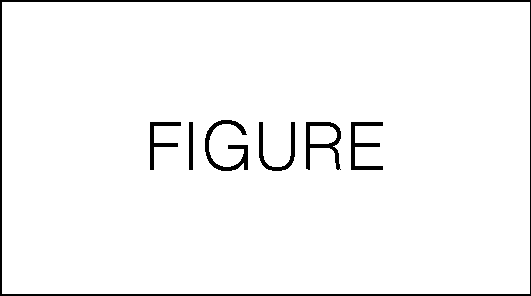
\includegraphics[width=0.7\textwidth]{DRAFT_FigsAndDocs/FIG}
	%%
	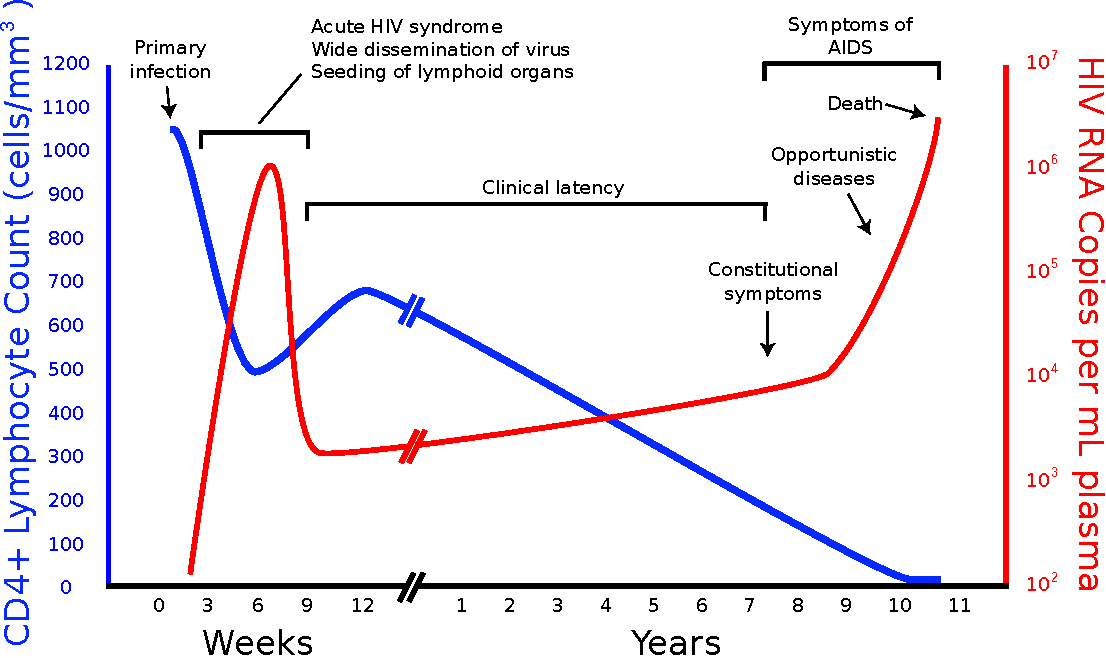
\includegraphics[width=14cm]{Figures/PrEP/HIV/HIVinfection}
	\captionsetup{width=0.85\textwidth}
	\caption[The HIV infection progression]{%
	{\bf The HIV infection progression}\\
	Average CD4+ T cell count (blue) and HIV viral load (red) during the course of an untreated HIV infection.  Image source: \cite[]{FigHIV} (no copyright).}
	\label{fig:PrEP_HIVstages}
\end{figure}

HIV infection may be diagnosed 10 to 90 days after exposure to HIV, depending on the testing method used~\cite[]{CDC_HIV}. To date, there is no cure for HIV. However, effective antiretroviral therapy (ART) inhibiting viral replication has been developed to treat HIV infection, stopping its progression. Multiple types of ART disrupting with different stages of the HIV life cycle are currently available. This has allowed to combine two or three different drugs, which is called combination ART, to prevent the emergence of drug resistance, which may result from the rapid mutation capacity of HIV~\cite[]{WHO_ART2016}.

The WHO currently recommends HIV infected individuals to start ART immediately after diagnosis, and to take ART for life~\cite[]{WHO_ART2016}. An infected individual successfully undergoing ART is able to decrease the viral load until being undetectable to HIV tests, which is called {\it viral suppression}. It has been shown in clinical trials that an individual with undetectable viral load does not transmit HIV~\cite[]{Rodger2016}. Moreover, the life expectancy for infected individuals taking ART can be almost the same as the life expectancy of uninfected individuals, especially in high-income settings~\cite[]{ARTCC2017}. Hence, thanks to effective ART, the number of infections, AIDS-related diseases and deaths has been greatly reduced globally~\cite[]{WHO_ART2016}.

\subsubsection*{The HIV epidemiology, worldwide}
The first patients with ---what would later be known as--- AIDS were observed in 1981~\cite[]{BarreSinoussi2013}. HIV was first isolated in 1983, and identified as its causal pathogen in 1984~\cite[]{Gallo2013}. The peak of the epidemic was observed in the late 90's. Nowadays, despite great efforts to prevent and treat HIV infection, the epidemic continues to spread globally~\cite[]{UNAIDS_Data2018,OWID}; see~\figref{fig:PrEP_HIVworld}. As of 2019, about 38 million people around the globe were living with HIV, and 32 million have died from AIDS-related illnesses since the start of the epidemic~\cite[]{UNAIDS_Factsheet2019}.

\begin{figure}[H]
	\centering
	%% DRAFT
%	\vspace{2cm}
%	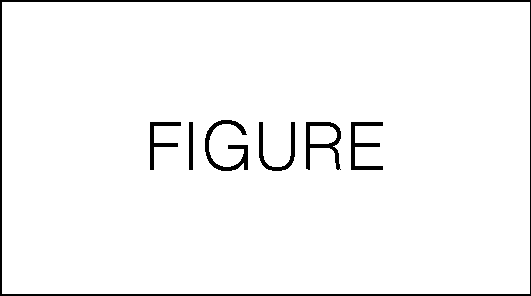
\includegraphics[width=0.9\textwidth]{DRAFT_FigsAndDocs/FIG}
	%%
	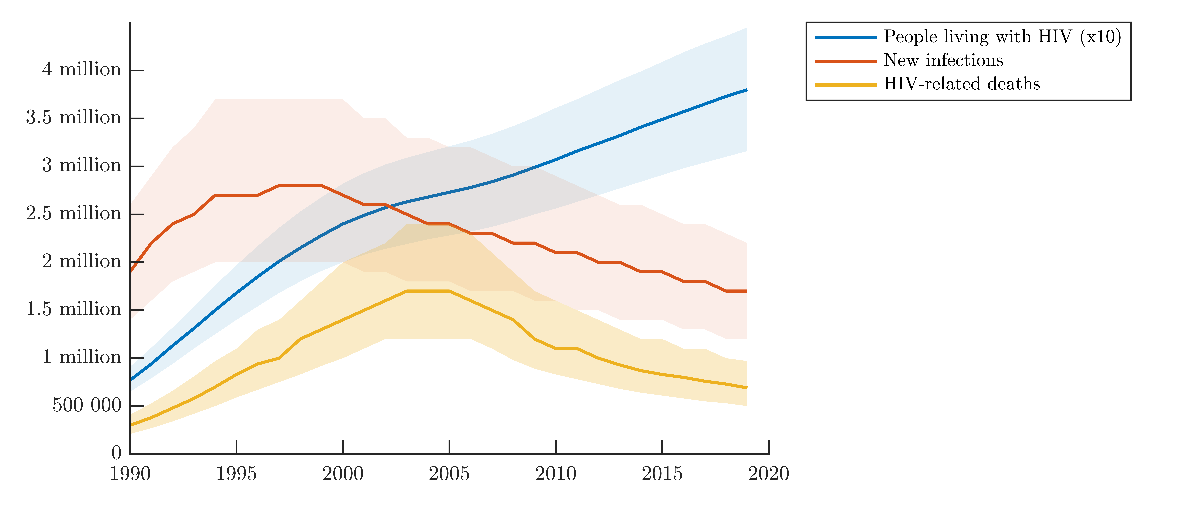
\includegraphics[width=16cm]{Figures/PrEP/HIV/HIV_Data_Global}
	\captionsetup{width=0.85\textwidth}
	\caption[HIV/AIDS epidemiological indicators, worldwide]{%
		{\bf HIV/AIDS epidemiological indicators, worldwide}\\
	Total number of people living with HIV (the data was divided by 10 to fit the same figure with the other mesures; i.e., in 2019, there were $\sim38$ million people living with HIV), number of new HIV infections and number of HIV-related deaths, from 1990 to 2019, worldwide.  Source: UNAIDS HIV estimates~\cite[]{UNAIDS_DataSpreadsheet}.}
	\label{fig:PrEP_HIVworld}
\end{figure}

%\subsubsection*{The HIV epidemic among men who have sex with men}

In most high-income settings, the HIV epidemic continues to expand among men who have sex with men (MSM)~\cite[]{UNAIDS_Data2018,WHO_KeyPop2016,Beyrer2012}. The high transmission of HIV among MSM may be explained by biological factors, such as the high probability of HIV transmission through receptive anal intercourse, as well as by behavioral factors, such as unprotected sexual intercourses, large number of casual partners and using recreational drugs~\cite[]{Beyrer2012}.

\subsubsection*{The prevention of HIV infection}

Prevention interventions have proven to be successful to reach risk reduction among MSM, by sharing information on HIV/AIDS risk, promoting safer sex and changes  in social behavior, etc.~\cite[]{Johnson2002}. The prevention methods against HIV include, among others: abstinence, condom use~\cite[]{Chen2017}, seroadaptation\footnote{The term {\it seroadaptation} refers to the adaptation of sexual behaviors due to serological status awareness. Similarly, {\it seropositive} (respectively, {\it seronegative}) refers to an individual infected (respectively, uninfected) with HIV.} (practices aiming to reduce contamination among serodiscordant sexual partners, such as seropositioning and serosorting)~\cite[]{McFarland2011,Velter2015} and, more recently, the use of ART as prevention (in the form of pre- and post-exposure prophylaxis)~\cite[]{WHO_ART2016}. 

\subsection{Pre-exposure prophylaxis}
%\subsection{Pre-exposure prophylaxis uptake among MSM}

Pre-exposure prophylaxis (PrEP) consists of the use of ART by uninfected individuals before possible exposure to HIV. The first commercialized version of PrEP consists of the combination of two antiretrovirals, Emtricitabine (FTC) and Tenofovir disoproxil fumarate (TDC), sold under the registered name Truvada\textsuperscript{\textregistered}, and currently available in generic form. FTC/TDC pills may be taken continuously (i.e., taken every day) or \textit{on demand} (i.e., taken right before and after possible exposure to HIV)~\cite[]{Desai2018,Siguier2018}. %New ART combinations and new means of administration are currently to be used as PrEP~\cite[]{Siguier2018}.

Hopes are that the use of PrEP may curb the HIV epidemic among MSM. Recent studies have estimated a reduction in the number of new HIV infections at the population level after PrEP rollout among high-risk MSM that may place some settings in the path towards HIV epidemic elimination~\cite[]{Palk2018,Grulich2018,Brown2018}.

\subsubsection*{Efficacy of PrEP}

The first randomized, double blind, clinical trial conducted among MSM to study the efficacy of PrEP was the \textit{iPrex} study, which showed a moderate relative risk reduction of 44\%, through daily use of TDF-FTC (versus placebo)~\cite[]{Siguier2018,Grant2010}. However, the results suggested that compliance was a major factor for efficacy: the risk reduction increased to 92\% when considering only the subgroup of individuals with detectable TDF-FTC concentrations~\cite[]{Grant2010}.

The efficacy of daily oral PrEP was also studied among serodiscordant heterosexual couples in the \textit{Partners} study, which found a TDF-FTC PrEP efficacy of 84\% for men and 66\% for women, and in the \textit{TDF-2} study, where the efficacy was estimated at 62.2\%~\cite[]{Siguier2018}. Among heterosexual women, two studies found no efficacy of PrEP, due to the low compliance of the participants~\cite[]{Siguier2018}. An efficacy of 49\% was estimated at a study among injecting drug users~\cite[]{Siguier2018}.

Two recent trials conducted on high-risk MSM showed that PrEP has an effectiveness of 86\%; \textit{PROUD}, a study comparing daily PrEP uptake versus the deferred (by 1 year) adoption of daily PrEP~\cite[]{McCormack2016}, and \textit{Ipergay}~\cite[]{Molina2015}, a randomized double blind trial comparing on-demand PrEP uptake versus placebo. Both the placebo arm of \textit{Ipergay} and the deferred arm of \textit{PROUD} were discontinued anticipatedly, in light of the high efficacy of PrEP~\cite[]{Siguier2018}. The open-label follow-up of the participants of the \textit{Ipergay} trial showed a 97\% reduction in the incidence~\cite[]{Siguier2018,Molina2017}. In addition, two cohort studies observed no HIV infections among MSM taking PrEP under good compliance~\cite[]{Siguier2018,Desai2018}. These results place PrEP, next to condom use, among the most effective HIV prevention methods for MSM. 

Therefore, the WHO currently recommends PrEP as a prevention method for MSM at high risk of HIV of infection~\cite[]{WHO_StartART2015,WHO_KeyPop2016,WHO_ART2016}. Individual-level PrEP eligibility criteria for MSM include, for instance, having unprotected anal intercourses with casual partners and/or partners with positive or unknown serostatus~\cite[]{WHO_StartART2015}. PrEP uptake recommendations include providing PrEP together with other HIV prevention options (notably, condom use), performing HIV tests every 3 months, regularly testing for other STIs and monitoring renal functions~\cite[]{WHO_ART2016}

\subsubsection*{Price of PrEP and cost-effectiveness analyses}
The price payed by PrEP users varies widely between countries where PrEP is available. In the US, the price of PrEP may be about 1\,400\euro\, to 1\,800\euro\, per month, while in countries like France and Sweden, PrEP is offered for free to individuals, since it is completely covered or reimbursed by the social security system. In addition, the availability of generic TDF/FTC molecules has led to a reduction in the price of PrEP paid by individuals in countries like Germany, Ireland, Switzerland and Poland~\cite[]{TheBody_PrEPcost}. 

Cost-effectiveness analyses have shown that a PrEP rollout among MSM at high risk of infection is cost-effective in comparison to other interventions~\cite[]{DurandZaleski2018,Revill2017,Cambiano2017,Nichols2016,Ouellet2015,Desai2008}, but may remain expensive nevertheless~\cite[]{Juusola2013,Gomez2012}. Moreover, cost-effectiveness analyses have shown to be highly sensitive to the price of PrEP~\cite[]{Coleman2017}. This exhibits the need of reducing PrEP price, which remains a key barrier to broadly provide PrEP through public health programs~\cite[]{ECDC_PrEP2016}.

\subsubsection*{PrEP availability and accessibility}

As of June 2018, only 35 countries had at least one public policy implemented regarding PrEP rollout; most of them (15 countries) in the European region~\cite[]{HodgesMameletzis2018}. Global efforts thus remain far from the WHO recommendations to scale up PrEP programs among high-risk populations~\cite[]{WHO_KeyPop2016}. 



%\subsubsection*{PrEP-induced risk compensation}

\subsubsection*{PrEP acceptability among MSM}
As with other prevention methods, PrEP effectiveness is associated with persistence and adherence, which highlights the importance of MSM accepting to adopt and keep using PrEP as long as their risk of HIV infection remains high, and use it correctly. It is thus important for individuals to have a fair perception of their risk of HIV infection, the consequences of acquiring HIV infection and all the implications of a PrEP uptake to make informed decisions on whether or not to adopt PrEP as a prevention method against HIV infection. 

On the one hand, the MSM community has shown to be highly aware on their risk of infection, which has resulted in the practice of risk-reduction strategies~\cite[]{McFarland2011,Velter2015}. Paradoxically, these preventive practices may mislead individuals into believing their sexual behaviors are not risky enough~\cite[]{Golub2014}, so additional prevention measures such as PrEP may not be adopted~\cite[]{Young2014}. On the other hand, MSM have also shown to be highly aware of PrEP~\cite[]{Frankis2016,Grov2016} and PrEP has shown to be well-accepted (if available) among MSM who identify themselves at high risk of infection~\cite[]{Frankis2016,Ferrer2016,Taylor2014,Aghaizu2013}. 

Still, PrEP acceptability among MSM has been recently estimated at a moderate level of about 58\%~\cite[]{Peng2018}. Acceptability may be affected not only by the price of the molecule, but also by other non-monetary barriers, all the extra efforts and discomfort that the individuals on PrEP may confront; for instance: difficulties regarding PrEP uptake and accessibility, pill burden, difficulties in managing adherence, fear of acquiring other sexually transmitted infections due to drop in condom use~\cite[]{Young2014,Taylor2014,PerezFigueroa2015,Holt2018,Desai2018,Sidebottom2018}, difficulties understanding PrEP effectiveness~\cite[]{Underhill2016}, lack of tolerability~\cite[]{Siguier2018}, alcohol-PrEP interactive toxicity beliefs~\cite[]{Kalichman2017} and social stigma and discrimination~\cite[]{Young2014,PerezFigueroa2015,Arnold2016}.

% PrEP adherence and persistence. 

\subsection{The HIV epidemiology and PrEP rollout in France}
\label{PrEP:France}
%\subsection{The HIV epidemiology among French MSM and the rollout of PrEP in France}

In France, like in most high-income settings, the number of new HIV infections remains remarkably high in some subpopulations. Between 6\,000 and 7\,000 new HIV infections are estimated to occur each year at the national level~\cite[]{Marty2018}. These numbers have remained rather stable since 2011~\cite[]{Siguier2018,SPF_Rapport2019}. More than 40\% of the new HIV infections occur among people living in �le-de-France (\^IdF)---the Paris region, while only 19\% of the French population lives in this region~\cite[]{Marty2018}. 

About 43\% of the new HIV infections occur among MSM~\cite[]{Siguier2018}, while MSM represent less than 2\% of the general population~\cite[]{Bajos2008}---1.6\% when defining MSM as men who had at least one sexual intercourse with another man in the past twelve months and 4\% when defining MSM as men who had at least one sexual intercourse with another man in their lifetimes~\cite[]{Marty2018}. 
%
By far, MSM are the most affected by HIV in France, with HIV incidence rates ($\sim$1\%) more than 60-fold higher than the national level~\cite[]{Marty2018}. The incidence rate among high-risk MSM living in \^IdF has been estimated as high as 9\% in the \textit{Ipergay} trial~\cite[]{Molina2018}.

%\begin{figure}[H]
%	\centering
%	\frame{%
%	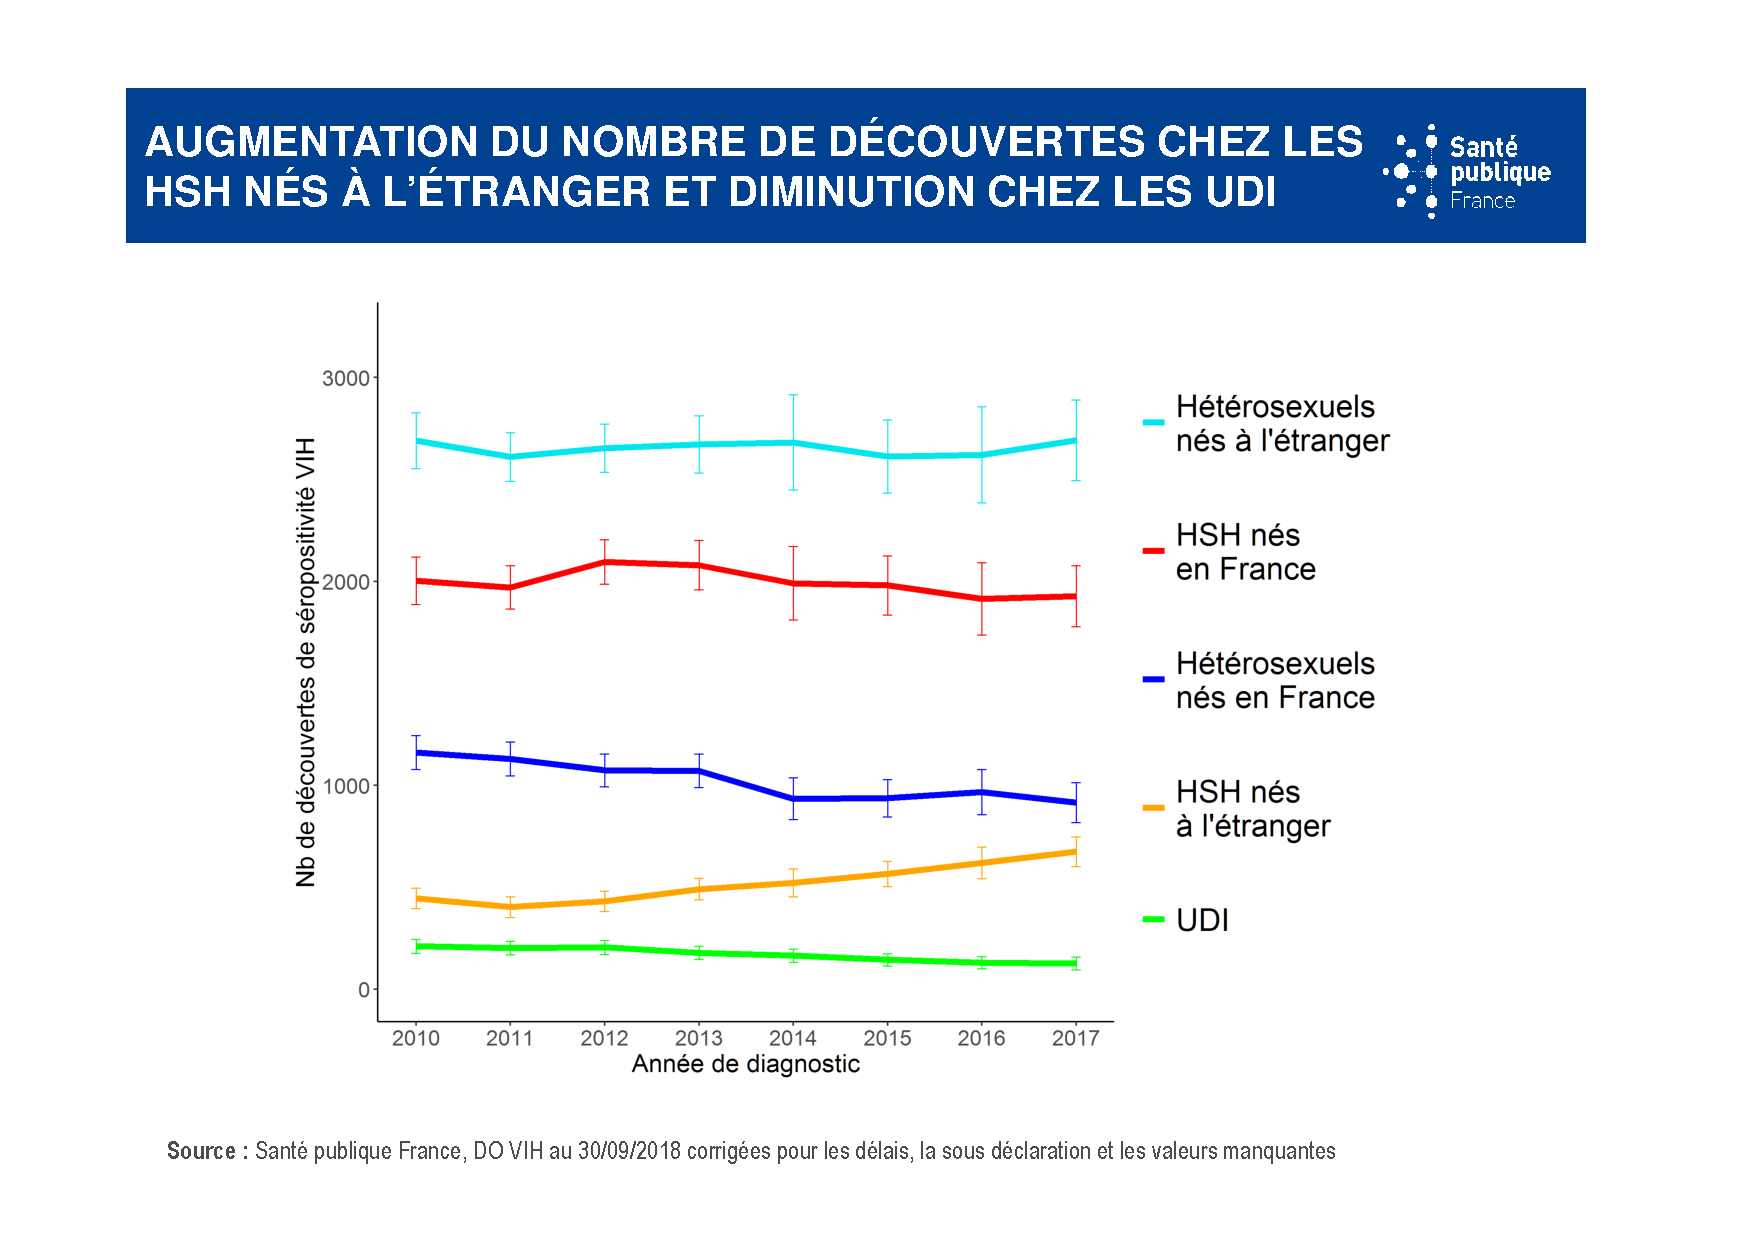
\includegraphics[height=8cm, trim=2cm 0 5cm 5cm,clip=true]{Figures/PrEP/HIV/VIH_France}
%	}
%	\captionsetup{width=0.85\textwidth}
%	\caption[New HIV infections in France]{%
%		{\bf New HIV infections in France}\\
%	Total number of new HIV infections in France.  Image source: Sant� Publique France~Ref.~\cite[]{SPF_VIHfr}.}
%	\label{fig:HIV_France}
%\end{figure}

%\subsubsection*{The HIV epidemic among MSM living in the Paris region}
%
%There were around 118\,000 MSM living in \^IdF (95\% confidence interval (CI): 83\,000--167\,000)~\cite[]{Bajos2008,Insee2015}. As of 2016, the mean prevalence was estimated at 16\% (95\% CI: 12\%--20\%)~\cite[]{Prevagay2017}, and 3\,400 (95\% CI: 3\,000--3\,800) MSM living with HIV were estimated to be unaware of their HIV status, each year (representing a 18\% (95\% CI: 15\%--20\%) of infected MSM)~\cite[]{Marty2019}. %The undiagnosed population is often referred to as the \textit{hidden epidemic}.
%%
%The yearly number of new HIV infections among MSM in \^IdF was estimated at 1\,100 (95\% CI: 900--1\,400), representing an overall mean incidence of 2\% (95\% CI: 1.0\%--2.6\%)~\cite[]{Marty2019}. The ANRS IPERGAY trial revealed an HIV incidence up to 9.2\% among MSM at high risk of HIV infection who lived in \^IdF~\cite[]{Molina2015,Molina2018}. 
%
%%We used this data to calibrate our transmission model (cf.~\hyperlink[Article2SM.14]{section 2} of the supplementary material).



\subsubsection*{PrEP rollout in France}

PrEP was authorized by French health authorities in 2016~\cite[]{Siguier2018} and is currently recommended for MSM at high risk of HIV infection~\cite[]{ANRS_VIH2015,ANSM_Truvada2017,Siguier2018,HAS_PrEP2019}. MSM need to meet at least one of the following criteria, to be prescribed PrEP:
\begin{itemize}
\item[i)] To have had unprotected, i.e., condomless sexual intercourses with at least 2 different partners in the last 6 months, 
\item[ii)] To have had STI events in the last 12 months;
\item[iii)] To have had at least one post-exposure treatment for HIV in the last 12 months;
\item[iv)] Drug use during sexual intercourse.
\end{itemize}

In France, the recommendation to use PrEP in its registered form (Truvada\textsuperscript{\textregistered}) was made in November 2015. Full PrEP reimbursement (both for Truvada and generics) by the French Social Security system was implemented in January 2016~\cite[]{ANSM_Truvada2017}. PrEP has also shown to be cost saving in the French context~\cite[]{DurandZaleski2018}. 

About 13\,900 MSM initiated PrEP in \^IdF between January 2016 and June 2020~\cite[]{ANSM_Truvada2020}, with a marked growing trend; cf.~\figref{fig:PrEP_IdF}. Still, there remains a gap between PrEP eligibility and PrEP adoption. A recent study found that there is a high number of missed opportunities of PrEP prescription (that is, cases of MSM recently diagnosed with HIV that would have been eligible to a PrEP prescription)~\cite[]{Lions2019}. 

Among on-PrEP MSM in the Paris region, some evidence of risk compensation (drop in condom use) has been observed~\cite[]{Molina2018}. Also, a 30-month dropout rate of $\sim 32\%$~\cite[]{Costagliola2019}, which reveals the need of understanding and addressing PrEP persistence.


%\begin{figure}[H]
%	\centering
%	\includegraphics[width=12cm]{Figures/PrEP/HIV/PrEP_Data_FR}
%	\captionsetup{width=0.85\textwidth}
%	\caption[PrEP users in France]{%
%		{\bf PrEP users in France}\\
%	Number of PrEP first prescriptions (i.e., people starting PrEP) at the national level, from January 1st, 2016 to June 30th, 2018. Total Source: National agency of medicine and health products safety (ANSM)~\cite[]{ANSM_Truvada2020}.}
%	\label{fig:PrEP_France}
%\end{figure}

\begin{figure}[H]
	\centering
	%% DRAFT
%	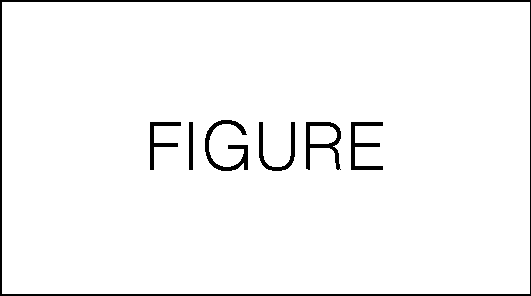
\includegraphics[width=0.7\textwidth]{DRAFT_FigsAndDocs/FIG}
	%%
	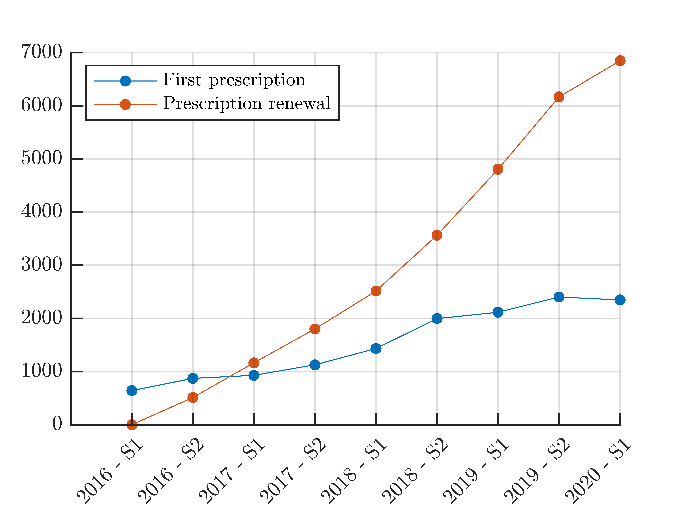
\includegraphics{Figures/PrEP/HIV/PrEP_Data_IDF}
	\captionsetup{width=0.85\textwidth}
	\caption[PrEP users in �le-de-France, by semester, by year]{%
		{\bf PrEP users in �le-de-France, by semester, by year}\\
	Number of first PrEP prescriptions (i.e., people starting PrEP; in blue) and PrEP prescription renewals (in red) in the Paris region, by semester (S1 and S2) from January 1st, 2016 to June 30th, 2020. The data suggested that the great majority of PrEP users in the region were MSM. The total number of first prescriptions since PrEP rollout in the region was $\sim13\,900$ while only $\sim6\,850$ prescription renewals were established the first semester of 2020. On average, 85\% of PrEP users got a prescription renewal the following year. Source:~\citet{ANSM_Truvada2019,ANSM_Truvada2020}\footnotemark.}
	\label{fig:PrEP_IdF}
\end{figure}

\footnotetext{Scientific group of the  French Agency of Medicine and Health Products Safety (ANSM) analyzing the data collected by the French System of Health Data (SNDS).}

\subsection{Worldwide efforts to end AIDS and the path towards ending the HIV epidemic}

Ending AIDS has become a global objective. Specific strategies and objectives have been set  during the past decade~\cite[]{UNAIDS_EndAIDS2011,UNAIDS_EndAIDS2030}. Nowadays, the initiative to end AIDS as a public health threat by 2030 is part of the Sustainable Development Goals. 
%
One essential direction adopted towards ending AIDS has been HIV prevention through the combination of behavioral and biomedical approaches~\cite[]{UNAIDS_EndAIDS2011,UNAIDS_EndAIDS2030}. In particular, the WHO has published recommendations targeting the populations most at risk of HIV infection\footnote{Also called {\it key populations}, among which an HIV incidence greater than 3 per 100 person-years has been observed~\cite[]{WHO_StartART2015}.}, which include MSM~\cite[]{WHO_KeyPop2016}. 
%
Another strategy to end AIDS is through the scaling up of diagnosis, treatment and care. The UNAIDS 90--90--90 initiative was launched in 2015, aiming for 90\% of infected individuals to be aware of their serostatus, 90\% of diagnosed individuals to receive sustained ART and 90\% of treated individuals to reach viral suppression, by 2020~\cite[]{UNAIDS_909090_2017}. In 2016, the objectives were extended to 95\%--95\%--95\% by 2030, targeting to achieve a 90\% reduction in HIV incidence compared with 2010 levels~\cite[]{UNAIDS_EndAIDS2030}. The reduction in the number of in \rev{TERMINAR}

\subsection{Mathematical modeling of the HIV epidemic and PrEP uptake among MSM}

Mathematical modeling has been extensively used to describe the HIV epidemic dynamics~\cite[]{Jacquez1988,CastilloChavez1989}. In particular, it has been used to describe HIV transmission among MSM and to evaluate the impact of preventive interventions on the epidemic's dynamics~\cite[]{Gumel2006,Gomez2012,Punyacharoensin2011,Eaton2012,Cremin2013,Punyacharoensin2016,Kim2014,Robineau2017,Palk2018,LeVasseur2018}. For instance, deterministic approaches using compartmental models have been implemented to describe the HIV transmission at the population level~\cite[]{Supervie2010,Punyacharoensin2011,Gomez2012,Juusola2013,Kim2014,Punyacharoensin2016,Palk2018,Rozhnova2018}.

The heterogeneity of the risk of HIV infection among MSM has been modeled by considering structured mixing, where the population is stratified by risk of infection and the probabilities of sexual contacts between individuals are assumed to be non-random~\cite[]{Jacquez1988,Jacquez1989,Gupta1989,Sattenspiel1990}. The risk categories have been defined according to the individuals sexual behavior: by explicitly defining the probabilities of HIV transmission in terms of the number of sexual contacts the individuals may sustain, the probability of having sexual contacts with individuals in other risk-categories and the inherent probability of HIV-transmission.\footnote{Sexual behavior is also referred to in the literature as {\it sexual activity}. Sexual contacts may be defined, for instance, by sex acts or sexual partnerships~\cite[]{Jacquez1988}.} Hence, an individual at high-risk (respectively, low-risk) of infection would be assumed to have a high (respectively, low) number of sexual contacts.

There are two main kinds of non-random structured mixing that have been used to model HIV-transmission dynamics: i) {\it proportional mixing}, where sexual contacts are assumed to be proportional to the number of individuals in each risk-category; and ii) {\it preferred mixing,\footnote{Also referred to as {\it assortative mixing}.}} where a fraction of the individuals is assumed to mix preferentially with other individuals in the same risk-category, and the rest of the contacts are proportional~\cite[]{Jacquez1988}. The higher the heterogeneity, the lower the prevalence at the endemic state (where there are no changes in the epidemic dynamics) and, in the case that extremely risky behaviors are considered, two peaks may be observed in the epidemic dynamics~\cite[]{Punyacharoensin2011}.

Modeling studies have evaluated the impact of a PrEP rollout on the HIV epidemic among MSM, predicting a remarkable reduction in the number of new HIV infections~\cite[]{Gomez2012,Kim2014,Punyacharoensin2016,Jenness2016,Robineau2017,Rozhnova2018,Palk2018,Rozhnova2019}. In particular, recent mathematical models have studied HIV epidemic elimination through PrEP rollouts among MSM~\cite[]{Rozhnova2018,Scott2018,Hansson2020}. These models assume that PrEP coverage can reach any value and, in particular, high values, which may not be granted in the real world. Therefore, it is unclear whether and how PrEP coverage levels, which are required to substantially impact or eliminate HIV epidemics, can be reached and maintained, in the long term. 

The subject of HIV elimination through healthcare interventions has also been addressed by modeling studies. For instance, by defining HIV elimination as the effective reproduction number being below 1, along with an incidence under 1 yearly case by 1000 individuals, a 2009 study found that testing the whole population yearly and treating immediately all seropositive individuals may result in epidemic elimination within 10 years~\cite[]{Granich2009}. Another 
study found that, to reach less than 1 yearly case by 1000 among MSM in the UK, would require a 90\% of recently infected individuals to be diagnosed and treated in the year following infection~\cite[]{Phillips2013}. A more recent study estimated that, reaching the 95--95--95 target, along with high adoption of preventive methods like PrEP and condom coverage among MSM, would only ensure an 80\% reduction in incidence by 2030~\cite[]{Scott2018}. Regarding PrEP interventions, a recent study found that HIV elimination would require $82\%$ PrEP coverage among high-risk MSM during 5 years to reach HIV elimination~\cite[]{Rozhnova2018}.

To the best of our knowledge, no modeling study has addressed the individual-level decision-making on whether or not to adopt a prevention method---namely, PrEP---to avoid HIV infection and thus evaluated the impact of voluntary adoption of PrEP on the HIV epidemic. 


\section{Objectives}
\label{PrEP:Objective}
The main objective of the second part of my PhD was to model HIV transmission within the population of MSM, taking into account the individual-level decision-making on whether or not to adopt PrEP as a prevention method against HIV, in the current therapeutic context. To that end, we built a mathematical model describing the HIV transmission at the population level, coupled with a model accounting for the individual-level dilemma of prevention versus treatment regarding PrEP. In particular, we aimed to address this issue for one of the most at risk populations in mainland France: MSM in �dF.

We aimed to obtain a mathematical characterization of the probability for a typical individual to adopt PrEP on his own, which would yield the voluntary PrEP coverage at the population level. Moreover, we expected to obtain the PrEP coverage as a function of the risk of HIV infection, the PrEP parameters and the HIV epidemic's intrinsic parameters (unlike previous studies, in which values are predetermined for the prevention coverage~\cite[]{Gomez2012,Punyacharoensin2016,Robineau2017,Rozhnova2018} or full PrEP coverage is assumed~\cite[]{Kim2014}). 

Finally, we aimed to evaluate the impact of PrEP on the HIV epidemic among MSM, when PrEP is taken voluntarily by those who find themselves most at risk. Moreover, we intended to determine whether and under what conditions could the voluntary PrEP coverage control and, eventually, eliminate the epidemic.


%\section{Published article}
\section{Article submitted for publication}
\label{PrEP:Article}
A scientific article presenting our findings, titled ``Can HIV epidemics among men who have sex with men be eliminated through participation to PrEP rollouts?''~\cite[]{Jijon2021}, \rev{was submitted for publication to the \emph{AIDS} journal in January 2021, and is currently under review}. 

The preprint of the main text is included below, along with the supplementary material, where the mathematics of our model is presented in detail. The computations and proofs of the analytical results presented in the article's supplementary material are available in~\secref{PrEP:AdditionalMaterial} of this chapter. A few additional figures are also found in~\secref{PrEP:AdditionalMaterial}. The implementation of HIV prevention programs are further discussed in~\secref{PrEP:Discussion}, as well as the limitations and perspectives of our modeling choices. 

\subsection{Description of the article}

We propose a mathematical model describing the interplay between the HIV epidemic among MSM and the individual-level decision-making on whether or not to adopt PrEP as a prevention method against HIV infection, in the current therapeutic context, where universal effective ART is in place. In particular, we addressed this issue for one of the most at risk populations in mainland France: MSM in \^IdF (the Paris region).

%The mixed model consist of a model describing the HIV transmission at the population level, coupled with a model accounting for the individual-level dilemma of prevention versus treatment regarding PrEP. 

\subsection{Results statement}
\label{PrEP:Results}

We obtained a mathematical characterization of the probability for a typical individual to adopt PrEP on his own, which would yield the voluntary PrEP coverage at the population level. We thus obtained the PrEP coverage reached voluntarily by high-risk MSM, as a function of the risk of HIV infection, the PrEP parameters and the HIV epidemic's intrinsic parameters, unlike previous studies, in which values are predetermined for the prevention coverage~\cite[]{Gomez2012,Punyacharoensin2016,Robineau2017,Rozhnova2018} or full PrEP coverage is assumed~\cite[]{Kim2014}. In particular, we study the PrEP coverage in terms of the PrEP effectiveness and the relative cost of PrEP versus ART perceived by individuals. 

We evaluated the impact of PrEP on the HIV epidemic among MSM, when PrEP is taken voluntarily by those who find themselves most at risk. Moreover, we identified the conditions for which epidemic control (i.e., reduction in HIV incidence) or elimination (i.e., reduction of HIV incidence to zero) are possible owing to voluntary adoption of PrEP by MSM at high risk of HIV infection in a typical urban setting of a high-income country (e.g., the Paris region). 

According to our findings, risk compensation (the reduction in condom use with PrEP adoption) may not play an essential role against epidemic elimination because PrEP is highly effective. However, several conditions regarding the relative cost of PrEP versus ART and risk perception need to be fulfilled to reach elimination. Specifically, the relative cost must be perceived by eligible MSM as sufficiently low, and the perception of the risk of acquiring HIV infection should be fair; if risk is underestimated, an even lower cost of PrEP is required for elimination. In addition, we found that lower testing rates among PrEP users require PrEP effectiveness to be high, in order to ensure epidemic elimination. Importantly, and similarly to our previous work on voluntary vaccination~\cite[]{Jijon2017}, we found that epidemic elimination is temporary unless active maintenance of the PrEP rollout is in place.

We conclude that current PrEP rollout protocols, including that of the Paris region, may not reduce enough the cost of PrEP to achieve epidemic elimination. Active efforts are thus needed to increase PrEP demand by easing PrEP access, identifying MSM at high risk of infection, and communicating HIV risk information to the target population. If these efforts lead to HIV elimination, the next challenge will be to maintain, in a context of less epidemic adversity, a low perception of the cost of PrEP and a fair perception of the HIV risk. 

%\newpage
%%%
%%% Article
%%%
%\includepdf[pages = -,
%		addtotoc = {1,subsection,1,Article,articlepdf:2},
%		addtolist = {
%                       	30, figure, {The voluntary PrEP coverage and its impact on HIV incidence, assuming fair risk perception}, fig:PrEP_1,
%			31, figure, The probability of HIV elimination and boundary uncertainty for the three-regions structure, fig:PrEP_2,
%                       	32, figure, Sensitivity analyses for the baseline scenario, fig:PrEP_3},
%		frame = false,
%		link = true,
%		linkname = Article2,
%		offset = 0cm -0.5cm,
%		openright = false,
%		pagecommand = {},
%		pages=-,
%		height = 25cm]
%		{Parts/Documents/Article2_PrEP}
%%		{DRAFT_FigsAndDocs/DOC.pdf}
%
%%%
%%% Article's Supplementary material
%%%
%\includepdf[pages = -,
%		addtotoc = {1,subsection,1,Supplementary material,articlepdf:2_SM},
%		addtolist = {
%			15, table, Initial values for several epidemiological indicators about the MSM population in the Paris region, table:PrEP_S3,
%			16, table, {Definition, initial value and calibrated values for the model parameters}, table:PrEP_S4,
%			17, table, Calibration to the HIV epidemiology for MSM in the Paris region, table:PrEP_S1,
%			17, table, Epidemiological indicators for the HIV transmission model at the endemic state, 	table:PrEP_S2,
%                       	18, figure, {Flow diagram for the compartmental model of HIV transmission among MSM, when PrEP is not available as a prevention method}, fig:PrEP_S1,
%			19, figure, {Flow diagram for the compartmental model of HIV transmission among MSM, when PrEP is available as a prevention method}, fig:PrEP_S2,
%			20, figure, The effective reproduction number $R$ as a function of the PrEP parameters, fig:PrEP_S3,
%			21, figure, {Impact of rollout with voluntary PrRP uptake, function of the relative cost of PrEP versus ART, when the PrEP effectiveness is 86\%}, fig:PrEP_S5,
%			22, figure, Impact of risk compensation on the voluntary PrEP coverage, fig:PrEP_S7},
%		frame = false,
%		link = true,
%		linkname=Article2SM,
%		offset = 0cm -0.5cm,
%		openright = false, 
%		pagecommand = { },
%		height = 27cm]
%		{Parts/Documents/Article2_PrEP_Appendix}


\section{Additional material} 
\label{PrEP:AdditionalMaterial}

Here, we present the computations and proofs of the results shown in the article's supplementary material (cf.~\secref{PrEP:Computations}). Namely, the explicit computations of some epidemiological indicators, using the ODE system (see sections~\ref{sec:Comp_PrEPeffectiveness}--\ref{sec:Comp_R}), the thresholds for the PrEP effectiveness and the perceived relative cost yielding epidemic control and elimination (see sections~\ref{sec:Comp_EpiControl}--\ref{sec:Comp_EpiElim} and~\ref{sec:Comp_rCrE}), and a description of the numerical approximation of the voluntary PrEP coverage (see~\secref{sec:Comp_VolPrEP}). 

This section also contains some additional figures that where not included in the paper submission, but may help visualizing the system behavior from other perspectives (cf.~\secref{PrEP:AdditionalFigures}). For instance, we present the values of the reproduction number before PrEP introduction for the calibrated model (see~\figref{fig:PrEP_R0} in~\secref{sec:R0}) and the number of HIV infections among on-PrEP MSM ---despite PrEP adoption--- for the baseline scenario (that is, assuming that individuals have a fair perception of HIV risk, a PrEP-induced condom drop from 30\% to 20\% and a 3-monthly HIV testing rate among on-PrEP MSM; see~\figref{fig:InfectionsOnPrEP} in~\secref{sec:InfOnPrEP}). Some additional figures and results for the scenario where on-PrEP MSM do not follow the recommendations on frequently testing for HIV are presented as well (see~figs.\ref{fig:SA_phi}--\ref{fig:SA_ProbElim} in~\secref{sec:FigsSensAnal}).


\subsection{Computations and proofs of our analytical results} 
\label{PrEP:Computations}

\subsubsection*{The effectiveness of PrEP}
\addcontentsline{toc}{subsubsection}{The effectiveness of PrEP}
\label{sec:Comp_PrEPeffectiveness}

PrEP effectiveness has been estimated at 86\% (95\% CI: 40\%--98\%) in two clinical trials conducted among MSM~\cite[]{Molina2015,McCormack2016} and at 85\%--96\% in simulation studies~\cite[]{Dimitrov2019}, using the PrEP-induced relative reduction of the HIV incidence,
\[
1-\frac{\text{HIV incidence with PrEP}}{\text{HIV incidence without PrEP}}.
\]

Here, we analyze a simplified version of our HIV transmission model (cf. eqs.~\hyperlink{Article2supp.5}{(S6)}) that mimics the IPERGAY trial~\cite[]{Molina2018}, in order to estimate the parameter representing the effectiveness of PrEP,~$\varepsilon$. 

We consider the population at high risk of infection, exclusively. We use $Q$ to denote the individuals in the control group and $P$ to denote the individuals using PrEP.  We suppose the control group and the study group are matched and use $\Lambda$ to denote their force of infection. Then, the following ODE system models the HIV infections dynamics that occur during the study:
\begin{align}
	\label{eq:IPERGAYmodel_1} \frac{dQ}{dt} &= - \Lambda Q,\\
	\label{eq:IPERGAYmodel_2} \frac{dP}{dt} &= - (1-\varepsilon) \Lambda P.
\end{align}

We use $\tau$ to denote the duration of the study follow-up. Dividing~\eqref{eq:IPERGAYmodel_1} by~\eqref{eq:IPERGAYmodel_2}, and integrating on the interval $[0,\tau]$, we obtain
\begin{equation} \label{eq:IPERGAY_ODE}
	\int_0^\tau \frac{dQ}{Q} = \int_0^\tau \frac{dP}{(1-\varepsilon) P}.
\end{equation}
We solve~\eqref{eq:IPERGAY_ODE} for the PrEP effectiveness, $\varepsilon$:
\begin{equation}
	\varepsilon = 1 - \frac{\ln P(\tau) - \ln P(0)}{\ln Q(\tau) - \ln Q(0)}.
\end{equation}
Using the number of participants and the number of seroconversions that took place during the ANRS IPERGAY study~\cite[]{Molina2015},
\begin{equation}
\begin{aligned}
	P(0) = 199, \qquad 	Q(0) = 201,\\
	P(\tau) = 197, \qquad 	Q(\tau) = 187,
\end{aligned}
\end{equation}
we have $\varepsilon = 0.86$. Hence, we found a value equivalent to the efficacy estimated in from the ANRS IPERGAY trial, corroborating our modeling choices in \hyperlink{Article2supp.5}{section 1.2} of the article's appendix.



\subsubsection*{The disease-free equilibrium}
\addcontentsline{toc}{subsubsection}{The disease-free equilibrium}
\label{sec:Comp_DFS}

The disease-free state (DFS) of the ODE system~\hyperlink{Article2supp.5}{(S6)} is given by 
\begin{equation} \label{eq:S_DFS}    
	P^{\rm DFS} = \frac{\pi_h p}{\mu}, \qquad 
	S_h^{\rm DFS} = \frac{\pi_h (1-p)}{\mu},\qquad
	S_\ell^{\rm DFS} = \frac{\pi_\ell}{\mu},
\end{equation}
and 
\begin{equation} \label{eq:I_DFS}
    I_i^{k,\rm DFS} =  T_i^{\rm DFS} = 0, \qquad \text{for all } i\in\{h,\ell\}, k\in\{a,c\}.
\end{equation}

%The total populations at high and low risk of infection at the DFS are thus given by
%\begin{equation} \label{eq:N_i_DFS}
%	N_h^{\rm DFS}	= P^{\rm DFS} + S_h^{\rm DFS}= \frac{\pi_h}{\mu},
%	\qquad \text{and} \qquad
%	N_l^{\rm DFS}	= S_l^{\rm DFS} = \frac{\pi_\ell}{\mu},
%\end{equation}
%respectively. 
The total population at $i$ risk of infection at the DFS is thus given by $N_i^{\rm DFS} = \pi_i/\mu$, for $i\in\{h,\ell\}$. Then, the total population at the DFS is given by
\begin{equation} \label{eq:N_DFS}
	N^{\rm DFS} = N_h^{\rm DFS} + N_\ell^{\rm DFS} = \frac{\pi_h + \pi_\ell}{\mu}.
\end{equation}

Equations \eqref{eq:S_DFS}--\eqref{eq:N_DFS} are used to compute the effective reproduction number, below. %; see \secref{sec:Comp_R}.


\subsubsection*{Computing the effective reproduction number} 
\addcontentsline{toc}{subsubsection}{Computing the effective reproduction number} 
\label{sec:Comp_R}

To compute the effective reproduction number for the ODE system~{\normalfont \hyperlink{Article2supp.5}{(S6)}}, we follow the methods and notation presented in~\cite[]{VanDenDriessche2002}, where $R(p,\varepsilon)$ is defined as the larger eigenvalue of the \emph{next generation matrix}~\cite[]{VanDenDriessche2008,Diekmann1990}. 

We start considering the vector 
\begin{equation}
X=\left(
	\begin{array}c
	    I_P^a\\
	    I_h^a\\
            I_\ell^a\\
            I_P^c\\
            I_h^c\\
            I_\ell^c\\
            T_h\\
            T_\ell\\
            P\\
            S_h\\ 
            S_\ell	
	\end{array}
\right),
\end{equation}
where the first 8 compartments correspond to infected individuals. Then, we identify the vectors $\mathscr{F}$ and $\mathscr{V}$ (which represent the new infections and the transfers in and out of the compartments, respectively), satisfying $dX/dt = \mathscr{F} - \mathscr{V}$:

\begin{equation}
\mathscr{F}=\left(
    { \arraycolsep=6pt\def\arraystretch{1.3}
    \begin{array}c
	    (1-\varepsilon) \Lambda_P  P \\
	    \Lambda_h S_h \\
	    \Lambda_\ell S_\ell\\
	    0\\
	    0\\
	    0\\
	    0\\
	    0\\
	    0\\
	    0\\
	    0\\
    \end{array}
   }
\right),
\qquad
\mathscr{V}=\left(
    { \arraycolsep=6pt\def\arraystretch{1.3}
    \begin{array}c
	\left( \sigma_P + \theta_P+\mu \right) I_P^a \\
	\left( \sigma+\theta+\mu \right) I_h^a \\
	\left( \sigma+\theta+\mu \right) I_\ell^a \\
	- \sigma_P I_P^a + (\theta_P+\mu) I_P^c\\
	- \sigma I_h^a + (\theta+\mu) I_h^c \\
	- \sigma I_\ell^a + (\theta+\mu) I_\ell^c \\
	- \theta_P (I_P^a + I_P^c) - \theta \left(I_h^a + I_h^c \right) + \mu_T T_h \\
	- \theta \left(I_\ell^a + I_\ell^c\right) + \mu_T T_\ell \\
	- p \pi_h + \Big[ (1-\varepsilon) \Lambda_P  + \mu \Big] P \\
	- (1-p) \pi_h + \left( \Lambda_h + \mu \right) S_h \\ 
	- \pi_\ell + \left( \Lambda_\ell + \mu \right) S_\ell \\ 
    \end{array}
   }
\right).
\end{equation}

We use the subscript $n$ to denote the $n$-th entry of a vector and the subscript $nm$ to denote the $(n,m)$ entry of a matrix. 
%
The matrix $V$, with elements $V_{mn} = \partial \mathscr{V}_m/ \partial X_n \Big|_{\rm DFS}$, where $n,m=1,\ldots,8$, is given by
\begin{equation} \label{eq:matrixV}
V=\left(
\begin{array}{cccccccc}
\sigma +\theta_P +  \mu  & 0 & 0 & 0 & 0 & 0 & 0 & 0 \\
 0 & \sigma + \theta +\mu  & 0 & 0 & 0 & 0 & 0 & 0 \\
 0 & 0 & \sigma + \theta +\mu  & 0 & 0 & 0 & 0 & 0 \\
  -\sigma  & 0 & 0 & \theta_P + \mu & 0 & 0 & 0 & 0 \\
 0 & -\sigma  & 0 & 0 & \theta +\mu  & 0 & 0 & 0 \\
 0 & 0 & -\sigma  & 0 & 0 & \theta +\mu  & 0 & 0 \\
 -\theta_P & -\theta  & 0 & -\theta_P &  -\theta  & 0 & \mu_T& 0 \\
 0 & 0 & -\theta  & 0 & 0 & -\theta  & 0& \mu_T \\
\end{array}
\right),
\end{equation}
%\mbox{}\vfill
%and its inverse is given by
%\begin{equation} \label{eq:matrixVinv}
%V^{-1}=\left(
%	{ \arraycolsep=6pt\def\arraystretch{1.65}
%\begin{array}{cccccccc}
% \frac{1}{\mu +\theta _P+\sigma } & 0 & 0 & 0 & 0 & 0 & 0 & 0 \\
% 0 & \frac{1}{\theta +\mu +\sigma } & 0 & 0 & 0 & 0 & 0 & 0 \\
% 0 & 0 & \frac{1}{\theta +\mu +\sigma } & 0 & 0 & 0 & 0 & 0 \\
% \frac{\sigma }{\left(\mu +\theta _P\right) \left(\mu +\theta _P+\sigma
%   \right)} & 0 & 0 & \frac{1}{\mu +\theta _P} & 0 & 0 & 0 & 0 \\
% 0 & \frac{\sigma }{(\theta +\mu ) (\theta +\mu +\sigma )} & 0 & 0 &
%   \frac{1}{\theta +\mu } & 0 & 0 & 0 \\
% 0 & 0 & \frac{\sigma }{(\theta +\mu ) (\theta +\mu +\sigma )} & 0 & 0 &
%   \frac{1}{\theta +\mu } & 0 & 0 \\
% \frac{\theta _P}{\mu _T \left(\mu +\theta _P\right)} & \frac{\theta
%   }{(\theta +\mu ) \mu _T} & 0 & \frac{\theta _P}{\mu _T \left(\mu +\theta
%   _P\right)} & \frac{\theta }{(\theta +\mu ) \mu _T} & 0 & \frac{1}{\mu _T}
%   & 0 \\
% 0 & 0 & \frac{\theta }{(\theta +\mu ) \mu _T} & 0 & 0 & \frac{\theta
%   }{(\theta +\mu ) \mu _T} & 0 & \frac{1}{\mu _T} \\
%\end{array}
%    }
%\right).
%\end{equation}

Similarly, the elements of the matrix $F$ are defined as $F_{mn} = \partial \mathscr{F}_m/ \partial X_n \Big|_{\rm DFS}$. Therefore, we calculate the values for $ \partial \Lambda_i / \partial I_j^k$. Recalling the definition~(\hyperlink{Article2supp.5}{S5}), we have 
\begin{equation}
\begin{aligned}
	\Lambda_h & = \frac{\lambda_{hh}^a \left( I_P^a + I_h^a \right) + \lambda_{hh}^c \left( I_P^c + I_h^c\right)}{N_h} + \frac{\lambda_{\ell h}^a I_\ell^a + \lambda_{\ell h}^c I_\ell^c}{N_\ell},
	\end{aligned}
\end{equation}
and
\begin{equation}
\begin{aligned}
	\Lambda_\ell &= \frac{\lambda_{h\ell}^a \left( I_P^a + I_h^a \right) + \lambda_{h\ell}^c \left( I_P^c + I_h^c\right)}{N_h} + \frac{\lambda_{\ell \ell}^a I_\ell^a + \lambda_{\ell \ell}^c I_\ell^c}{N_\ell},
	\end{aligned}
\end{equation}
where $$\lambda_{ji}^k = c_i \rho_{ij} \beta_j^k,$$ for  $i,j \in \{h,\ell\}$ and $k \in \{a,c\}$.
%
Then,
\begin{equation} \label{eq:derLAMBDA_i}
	\frac{\partial \Lambda_i}{\partial I_j^k} = \frac{\lambda_{ji}^k}{N_j} - \sum_{m} \left(\frac{\lambda_{hi}^m  I_P^m + \lambda_{hi}^m  I_h^m}{N_h^2} + \frac{\lambda_{\ell i}^m  I_\ell^m}{N_\ell^2}\right),
\end{equation}
where the sum is considered for all the values of $m \in \{a,c\}$.
% \rev{
%\begin{equation} \label{eq:derLAMBDA_i}
%\begin{aligned}
%\frac{\partial \Lambda_i}{\partial I_j^k}& = \frac{\partial}{\partial I_j^k} \left( \sum_{m, n} \frac{\lambda_{ni}^m  I_n^m}{N_n} \right) \\
%							& = \sum_{m, n} \lambda_{ni}^m \left(\frac{N_n\frac{\partial I_n^m}{\partial I_j^k} - I_n^m}{N_n^2}\right)\\
%							& = \frac{\lambda_{ji}^k}{N_j} - \sum_{m, n}  \frac{\lambda_{ni}^m  I_n^m}{N_n^2}
%\end{aligned}
%\end{equation}
%where all the sums are considered for all the values of $n \in \{h,\ell,P\}$ and $m \in \{a,c\}$. }
%
Evaluating~\eqref{eq:derLAMBDA_i} at the DFS defined in eqs.~\eqref{eq:I_DFS} and \eqref{eq:N_DFS}, we get $	\partial \Lambda_i/\partial I_j^k  \Big|_{\rm DFS} = \lambda_{ji}^k \, \mu/\pi_j$.
%\begin{equation} \label{eq:derLambda_DFS}
%%	\frac{\partial \Lambda_i}{\partial I_j^k}  \Bigg|_{\rm DFS} = \frac{c_i \rho_{ij} \beta_j^k \mu}{\pi_j}.
%	\frac{\partial \Lambda_i}{\partial I_j^k}  \Bigg|_{\rm DFS} = \frac{\lambda_{ji}^k \, \mu}{\pi_j}.\end{equation}
%
Therefore,
\begin{equation}
%	\frac{\partial}{\partial I_j^k} \Big(\Lambda_hS_h + (1-\varepsilon) \Lambda_P  P\Big) \Bigg|_{\rm DFS} = \left(1-\varphi(\varepsilon) \, p \right) \left(\frac{c_h \rho_{h j} \pi_h \beta_j^k}{\pi_j}\right),
	\frac{\partial}{\partial I_j^k} \Big(\Lambda_hS_h + (1-\varepsilon) \Lambda_P  P\Big) \Bigg|_{\rm DFS} = \left(1-\varphi(\varepsilon) \, p \right) \left(\frac{\lambda_{jh}^k \pi_h}{\pi_j}\right),
\end{equation}
and
\begin{equation}
	    \frac{\partial}{\partial I_j^k} \Lambda_\ell S_\ell \Bigg|_{\rm DFS} = \frac{\lambda_{j\ell}^k \,  \pi_\ell}{\pi_j}.
%	    \frac{\partial}{\partial I_j^k} \Lambda_\ell S_\ell \Bigg|_{\rm DFS} = \frac{c_\ell \rho_{\ell j} \pi_\ell \beta_j^k}{\pi_j}.
\end{equation}


The matrix $F$ is thus given by
\begin{equation} \label{eq:matrixF}
%\tiny
{\scriptsize
F=\left(
    { \arraycolsep=6pt\def\arraystretch{1.5}
\begin{array}{cccccccc}
 p (1-\varepsilon) \phi  \lambda_{hh}^a & p (1-\varepsilon) \phi  \lambda_{hh}^a & p (1-\varepsilon) \phi  \lambda_{\ell h}^a \pi_h/\pi_l & p (1-\varepsilon) \phi \lambda_{h h}^c & p (1-\varepsilon) \phi  \lambda_{h h}^c & p (1-\varepsilon) \phi  \lambda_{\ell h}^c \pi_h/\pi_l & 0 & 0 \\
 (1-p) \lambda_{hh}^a & (1-p) \lambda_{hh}^a & (1-p) \lambda_{\ell h}^a \pi_h/\pi_l & (1-p) \lambda_{h h}^c & (1-p) \lambda_{h h}^c & (1-p) \lambda_{\ell h}^c \pi_h/\pi_l & 0 & 0 \\
 \lambda_{h \ell}^a \pi_l/\pi_h & \lambda_{h \ell}^a \pi_l/\pi_h & \lambda_{\ell \ell}^a & \lambda_{h \ell}^c\pi_l/\pi_h & \lambda_{h \ell}^c\pi_l/\pi_h & \lambda_{\ell \ell}^c  & 0 & 0 \\
 0 & 0 & 0 & 0 & 0 & 0 & 0 & 0 \\
 0 & 0 & 0 & 0 & 0 & 0 & 0 & 0 \\
 0 & 0 & 0 & 0 & 0 & 0 & 0 & 0 \\
 0 & 0 & 0 & 0 & 0 & 0 & 0 & 0 \\
 0 & 0 & 0 & 0 & 0 & 0 & 0 & 0 \\
\end{array}
}
\right)}
\end{equation}
where
 $$\phi = \left( \frac{1-\xi \eta_P}{1-\xi \eta_h}\right).$$


\subsubsection*{The PrEP effectiveness threshold for epidemic control}
\addcontentsline{toc}{subsubsection}{The PrEP effectiveness threshold for epidemic control}
\label{sec:Comp_EpiControl}

Epidemic control induced by PrEP uptake is defined by a reduction of the effective reproduction number due to PrEP adoption, i.e., $R(p,\varepsilon)<R(0,\varepsilon)$; see~\hyperlink{Article2supp.7}{section 1.2.3} of the article's appendix. Here, we study the monotony of the reproduction number $R(p,\varepsilon)$ with respect to the PrEP parameters, PrEP effectiveness, $\varepsilon$, and PrEP coverage, $p$, in order to find the conditions necessary and sufficient to have $R(p,\varepsilon)<R(0,\varepsilon)$. \\

\noindent \textbf{Regarding PrEP effectiveness}

\noindent Recall the definition of $R(\varepsilon,p)$; see~\hyperlink{Article2supp.7}{eqs. (S14)--(S20)} of the article's appendix. Since $A>0$, the function $R(p,\varepsilon)$ verifies $\partial R(p,\varepsilon)/\partial \varepsilon \leq 0$ if and only if
\begin{equation} \label{eq:depsilon_dR}
\left(\frac{\partial}{\partial \varepsilon} H(p,\varepsilon) \right) \left( 1 + \frac{\Big(H(p,\varepsilon) - M\Big) + 2B M}{\sqrt{ \left(H(p,\varepsilon) - M\right)^2 + 4 B H(p,\varepsilon) M}}\right) \leq 0.
\end{equation}
%
Indeed, we have $\partial H(p,\varepsilon)/\partial \varepsilon \leq 0$; and, on the other hand, $A>0$, $M>0$ and $B \geq 1$, so
\begin{equation} \label{eq:sign_sqrt}
	H(p,\varepsilon) + M ( 2B -1) + \sqrt{ \left(H(p,\varepsilon) - M\right)^2 + 4 B H(p,\varepsilon) M} \geq 0.\\
\end{equation}

Therefore, $\partial R(p,\varepsilon)/\partial \varepsilon \leq 0$; that is, the higher the level of PrEP effectiveness, the higher the reduction of the effective reproduction number. \\

\noindent \textbf{Regarding PrEP coverage}

\noindent Similarly, $\partial R(p,\varepsilon)/\partial p \leq 0$ if and only if
\begin{equation}
\begin{aligned}
	& \left(\frac{\partial}{\partial p} H(p,\varepsilon) \right) \left( 1 + \frac{(H(p,\varepsilon) - M) + 2B M}{\sqrt{ \left(H(p,\varepsilon) - M\right)^2 + 4 B H(p,\varepsilon) M}}\right) \leq 0.
\end{aligned}
\end{equation}

From \eqref{eq:sign_sqrt}, we have $\partial R(p,\varepsilon)/\partial p \leq 0$ if and only if 
\begin{equation} 
	\frac{\partial}{\partial p} H(p,\varepsilon) = - H_h + (1-\varepsilon) \left( \frac{1-\xi \eta_P}{1-\xi \eta_h}\right) H_P \leq 0;
\end{equation}
Hence, $\partial R(p,\varepsilon)/\partial p \leq 0$ if and only if $\varepsilon \geq \varepsilon_{\rm C}$, where
\begin{equation} \label{eq:epsilonC}
\begin{aligned}
 	\varepsilon_{\rm C} = 1 - \left( \frac{1-\xi \eta_h}{1-\xi \eta_P}\right) \left( \frac{H_h}{H_P} \right).
\end{aligned}
\end{equation}


\subsubsection*{The PrEP effectiveness threshold for epidemic elimination}
\addcontentsline{toc}{subsubsection}{The PrEP effectiveness threshold for epidemic elimination}
\label{sec:Comp_EpiElim}

Epidemic elimination is defined by $R(p,\varepsilon) \leq 1$; see~\hyperlink{Article2supp.7}{section 1.2.3} of the article. That is,
\begin{equation}
	A \Big[ H(p,\varepsilon) + M + \sqrt{ \left(H(p,\varepsilon) - M\right)^2 + 4 B H(p,\varepsilon) M}\Big] \leq 1.
\end{equation}
Therefore,  $R(p,\varepsilon) \leq 1$, is achieved if and only if $p \,\varphi(\varepsilon) \leq K$, where
\begin{equation} \label{def:phi}
	\varphi(\varepsilon) \equiv H_h - (1-\varepsilon) \left( \frac{1-\xi \eta_h}{1-\xi \eta_P}\right)H_P,
\end{equation}
is a function of PrEP and condom effectiveness, and 
\begin{equation} \label{eq:K}
	K \equiv H_h -  \left(L - \frac{1}{2A}\right) \left(\frac{1}{1- 2AL (B - 1)}\right)
\end{equation}
is a constant independent of the PrEP parameters.

In addition, assuming $p=1$, $R(1,\varepsilon) \leq 1$ if  and only if $\varphi(\varepsilon) \leq K$, which is equivalent to $\varepsilon > \varepsilon_{\rm E}$, where
\begin{equation} \label{eq:epsilon_E}
\begin{aligned}
	\varepsilon_{\rm E} %&\equiv \varepsilon_{\rm C} +  K \left( \frac{1-\xi \eta_h}{1-\xi \eta_P}\right) \left(\frac{1}{H_P}\right)\\
	&\equiv 1- \left( 1- \frac{K}{H_h}\right) (1-\varepsilon_{\rm C}).
\end{aligned}
\end{equation}
In other words, $\varepsilon_{\rm E}$ is the minimum value of PrEP effectiveness for which epidemic elimination is possible, provided that PrEP coverage verifies $ p \, \varphi(\varepsilon_{\rm E}) \leq K$. Hence, we say that $\varepsilon_{\rm E}$ is the threshold for the PrEP effectiveness above which epidemic elimination is possible.

Note that \eqref{eq:epsilonC} can also be obtained from setting $\varphi(\varepsilon)\geq0$. Therefore, $\varphi(\varepsilon)$ can be interpreted as the effectiveness of PrEP and condom altogether. This can be straightforwardly identified in the scenario where individuals do not change testing behavior, i.e., where $\theta=\theta_P$; see~\figref{fig:SA_phi} below.


\subsubsection*{The rescaled perceived costs for the PrEP-adoption strategies}
\addcontentsline{toc}{subsubsection}{The rescaled perceived costs for the PrEP-adoption strategies}

We expanded analytically the costs defined by integrals in~\hyperlink{Article2supp.8}{eqs.~(S26)--(S27)} of the article's appendix  
\begin{equation} \label{eq:C_NP}
	C_{\text{\tiny No-PrEP}}(p;\varepsilon) = \left\{
	\begin{aligned}
	& \,  L \, e^{-\Lambda_h^{\rm ES}(p;\varepsilon) L} + L_T \left(1- e^{-\Lambda_h^{\rm ES}(p;\varepsilon) L} \right) - \frac{1 - e^{-\Lambda_h^{\rm ES}(p;\varepsilon)L}}{\Lambda_h^{\rm ES}(p;\varepsilon)}, &\qquad& \text{if } R>1\\
	&0 , &\qquad& \text{if } R\leq1,
\end{aligned}
\right.
\end{equation}
and
\begin{equation} \label{eq:C_P}
	C_{\text{\tiny PrEP}}(p;\varepsilon,r) = \left\{
\begin{aligned}
r & \left(\frac{1 - e^{-(1-\varepsilon)\Lambda_P^{\rm ES}(p;\varepsilon) L}}{(1-\varepsilon)\Lambda_P^{\rm ES}(p;\varepsilon)} \right) + L \, e^{-\left((1-\varepsilon)\Lambda_P^{\rm ES}(p;\varepsilon)+ \theta \right)L} \\
					& \qquad +  L_T \left(1- e^{-(1-\varepsilon)\Lambda_P^{\rm ES}(p;\varepsilon) L}\right) - \frac{1 - e^{-(1-\varepsilon)\Lambda_P^{\rm ES}(p;\varepsilon) L}}{(1-\varepsilon)\Lambda_P^{\rm ES}(p;\varepsilon)}, &\qquad& \text{if } R>1\\
	& r L , &\qquad& \text{if } R\leq1.
\end{aligned}
\right.
\end{equation}
The equations above were used to compute the expected utility directly and efficiently, and not in its integral form; cf.~\algoref{algo:maxU}.  \\

%\subsection{Interpreting the numerical results from maximizing the utility}
% The numerical methods fails to compute the endemic state near the threshold $R^\ast =1$. 
% How did we interpret the numerical result.
%\begin{figure}[H]
%	\centering
%	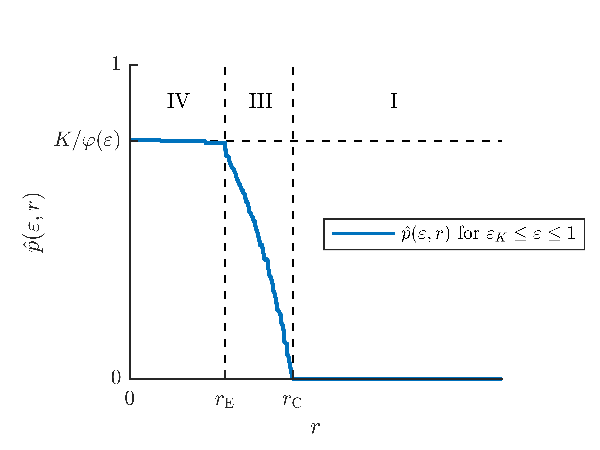
\includegraphics{Figures/PrEP/Results_Baseline/p_hat_num.pdf}
%	\caption[Numerical approximation of the voluntary PrEP coverage, for $\varepsilon \geq \varepsilon_{\rm E}$]{%
%	{\bf Numerical approximation of the voluntary PrEP coverage, for $\varepsilon \geq \varepsilon_{\rm E}$}\\
%	The explanation.
%	}
%	\label{fig:PrEP_phat_cut}
%\end{figure}


%\newpage
\subsubsection*{Numerical approximation of the voluntary PrEP coverage}
\addcontentsline{toc}{subsubsection}{Numerical approximation of the voluntary PrEP coverage}
\label{sec:Comp_VolPrEP}

The voluntary PrEP coverage was obtained numerically, as detailed in the \algoref{algo:maxU} below.

\begin{algorithm}[H]
\small
\caption{Numerical approximation of the voluntary PrEP coverage}
\label{algo:maxU}
\begin{algorithmic}[1]	
\Require Set of parameters for HIV transmission, small $\delta<0$.
\Ensure The voluntary PrEP coverage, $\hat{p}(\varepsilon,r)$
\Statex
        	\Procedure {Endemic force of infection, $\Lambda_i^{\rm ES}$}{$p,\varepsilon$} for $i\in\{h,P\}$  	\Comment{We used parallel computation.}
        	\For {$0 \leq p \leq 1$}
        		\For {$0 \leq \varepsilon \leq 1$}
			\State Compute $R(p,\varepsilon)$; cf. \hyperlink{Article2supp.6}{eqs.~(S14)--(S20)}
			\If {$R(p,\varepsilon) > 1$}
				\State Set $T$
				\While {$\log \left(|\left(N(t)-N(t-1)\right)/N(t-1)|\right) > \delta$}
					\State Increase $T$
 	       				\State Solve ODE system~\hyperlink{Article2supp.5}{(S6)} until $t=T$
				\EndWhile   
%%% begin break
%	\Comment{...Continues in the next page.}
%\algstore{bkbreak}
%\end{algorithmic}
%\end{algorithm}
%%
%\addtocounter{algorithm}{-1}
%%
%\begin{algorithm}[h]
%\small
%\caption{Numerical approximation of the voluntary PrEP coverage (continuation)}
%\begin{algorithmic}[1]
%\algrestore{bkbreak}
%%% end break
				\State Endemic state (ES) $\leftarrow$ ODE system at $t=T$
				\State Compute $\Lambda_h^{\rm ES}(p,\varepsilon)$; see \hyperlink{Article2supp.6}{eq. (S9)}
			\Else
				\State $\Lambda_h^{\rm ES}(p,\varepsilon) =0$
			\EndIf
	    	\EndFor
        	\EndFor 
	\State Compute $\Lambda_P^{\rm ES}(p,\varepsilon)$; see \hyperlink{Article2supp.6}{eq. (S13)}
        	\EndProcedure
\Statex
	\Procedure {Utility maximization, $\max_p U$}{$p;\varepsilon,r$}
	\State Compute $U(p;\varepsilon,r)$; cf. \hyperlink{Article2supp.8}{eq. (S25)} and \eqsref{eq:C_NP}{eq:C_P}
	\For {$0 \leq r \leq 1$}
		\For {$0 \leq \varepsilon \leq 1$}
			\State $\hat{p} \leftarrow$ The value of $p$ for which $U(p,\varepsilon,r)$ attains its maximum
		\EndFor
	\EndFor
	\EndProcedure
%\Statex
\State {\bf Return} $\hat{p}(\varepsilon,r)$
\end{algorithmic}
\end{algorithm}


\subsubsection*{Identifying the thresholds in relative cost for epidemic control and elimination} 
\addcontentsline{toc}{subsubsection}{Identifying the thresholds in relative cost for epidemic control and elimination}
\label{sec:Comp_rCrE}

The relative cost thresholds for epidemic control and elimination, $r_{\rm C}(\varepsilon)$ and $r_{\rm E}(\varepsilon)$ (cf. \hyperlink{Article2supp.11}{section 3.2.1} of the article's appendix), were numerically extracted from $\hat{p}(\varepsilon,r)$, by identifying the boundaries between the regions; see~\figref{fig:PrEP_r_thresholds}. 

On the one hand, $r_{\rm C}(\varepsilon)$ is the boundary between region III and region II: we defined $r_{\rm C}(\varepsilon)$ as the lowest value of $r$ for which $\hat{p}(\varepsilon,r)=0$, for any given PrEP effectiveness level $\varepsilon$. On the other hand, $r_{\rm E}(\varepsilon)$ is the boundary between region II and region I. Therefore, we identified $r_{\rm E}(\varepsilon)$ as the highest value of $r$ for which the difference between $\hat{p}(\varepsilon,r)$ and the theoretical threshold for PrEP coverage to yield epidemic elimination, $K/\varphi(\varepsilon)$, was lower than the tolerance we set in our algorithm. See \algoref{algo:rCrE} below for the numerical implementation and~\figref{fig:PrEP_r_thresholds} for an illustration of $r_{\rm C}(\varepsilon)$ and $r_{\rm E}(\varepsilon)$ for the baseline scenario.\\

\begin{algorithm}
\small
\caption{Identifying the relative cost thresholds for epidemic control and epidemic elimination}%, $r_{\rm C(\varepsilon)}$ and $r_{\rm E}(\varepsilon)$}
\label{algo:rCrE}
\begin{algorithmic}[1]	
	\Require $\hat{p}(\varepsilon,r)$ and $\Delta p$, the discretization step of the interval $[0,1]$ of $p$.
	\Ensure $r_{\rm C}$ and $r_{\rm E}$
\Statex
	\For {$0 \leq \varepsilon \leq 1$}
		\State $r_{\rm C}(\varepsilon) \leftarrow$  The lowest value of $r$ for which $\hat{p}(\varepsilon,r)=0$
		\If{$\varepsilon < \varepsilon_{\rm E}$}
			\State $r_{\rm E}(\varepsilon) \leftarrow$ The highest value of $r$ for which $\hat{p}(\varepsilon,r)=1$
		\Else
			\State $r_{\rm E}(\varepsilon) \leftarrow$ The highest value of $r$ for which $|\hat{p}(\varepsilon,r)-K/\varphi(\varepsilon)| \leq \Delta p$
		\EndIf
	\EndFor
\Statex
	\State {\bf Return} $r_{\rm C}(\varepsilon)$ and $r_{\rm E}(\varepsilon)$
\end{algorithmic}
\end{algorithm}

\begin{figure}[H]
	\centering
	%% DRAFT
%	\vspace{2cm}
%	 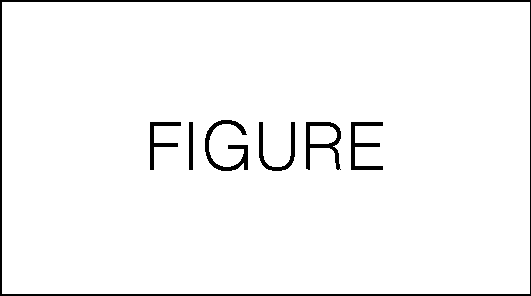
\includegraphics[width=0.7\textwidth]{DRAFT_FigsAndDocs/FIG}
	%%
	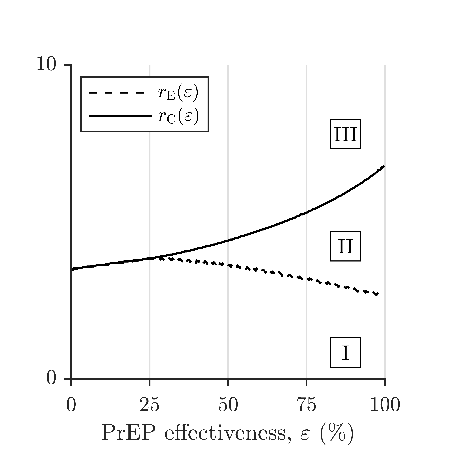
\includegraphics[width=8cm]{Figures/PrEP/Results_Baseline/rCrE}
	\caption[The relative cost thresholds for epidemic control and elimination]{%
	{\bf The relative cost thresholds for epidemic control and elimination}\\
	The relative cost thresholds for epidemic control and elimination as functions of PrEP effectiveness ($r_{\rm C}(\varepsilon)$ and $r_{\rm E}(\varepsilon)$, respectively) assuming fair perception of the risk of HIV infection, for a typical parameter set calibrating our model; see~\hyperlink{Article2supp.12}{table~S4} of the article's appendix. $r_{\rm C}(\varepsilon)$ is the boundary between region III and region II, while $r_{\rm E}(\varepsilon)$ is the boundary between region II and region I.}
	\label{fig:PrEP_r_thresholds}
\end{figure}



\subsection{Additional results and figures}
\label{PrEP:AdditionalFigures}

\subsubsection*{The effective reproduction number in the absence of PrEP}
\addcontentsline{toc}{subsubsection}{The effective reproduction number in the absence of PrEP}
\label{sec:R0}

We computed the effective reproduction number in the absence of PrEP, i.e., $R(0,0)$, for the $\sim500$ simulations calibrating our model; see~\figref{fig:PrEP_R0} below. We obtained a mean value of 2.2 (95\%~CI: 1.7--2.6). The values resulting from our model calibration are broadly in agreement with previous studies where $R_0$ has been estimated at 2--5 among MSM~\cite[]{Anderson1991}.
%$~2.29$~\cite[]{Stadler2012}. ????

\begin{figure}[H]
	\centering
	%% DRAFT
%	\vspace{1cm}
%	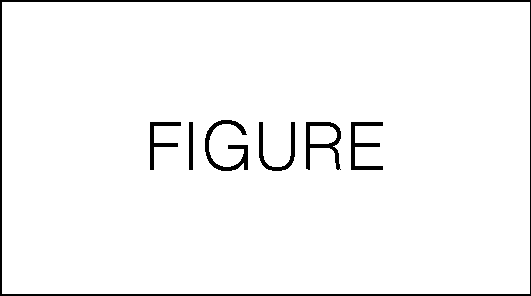
\includegraphics[width=0.7\textwidth]{DRAFT_FigsAndDocs/FIG}
	%%
	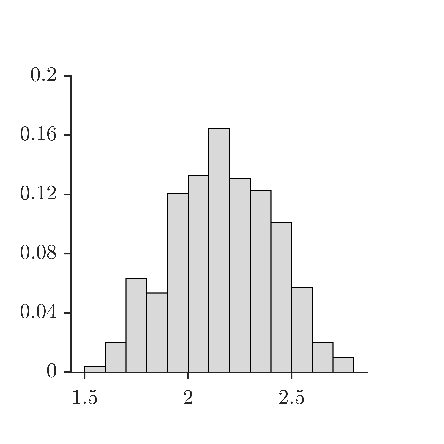
\includegraphics{Figures/PrEP/Results_Baseline/R0}
	\caption[The effective reproduction number in the absence of PrEP]{%
	{\bf The effective reproduction number in the absence of PrEP}\\
	Histogram of the values for the effective reproduction number in the absence of PrEP, $R(0,\varepsilon)$, for any value of PrEP effectiveness, $\varepsilon \in [0,1]$ and for the calibrated parameters sets; see~\hyperlink{Article2SM.16}{table~S2} of the article's appendix. The mean $R(0,\varepsilon)$ is 2.2 (95\%~CI: 1.7--2.6).}
	\label{fig:PrEP_R0}
\end{figure}


\subsubsection*{The number of new HIV infections despite PrEP uptake}
\addcontentsline{toc}{subsubsection}{The number of new HIV infections despite PrEP uptake}
\label{sec:InfOnPrEP}

In the baseline scenario, we assumed that on-PrEP MSM incur in risk compensation, decreasing their condom use from $30\%$ to $20\%$. The impact of risk compensation can be clearly seen in~\figref{fig:InfectionsOnPrEP}, which shows the number of new infections among on-PrEP MSM at the endemic state (ES), given by $(1-\varepsilon) \Lambda_P^{\rm ES}P^{\rm ES} = (1-\varepsilon) (1-\xi \eta_P)\Lambda_h^{\rm ES}P^{\rm ES} /(1-\xi \eta_h) $, where $\Lambda_P^{\rm ES}$ and $P^{\rm ES}$ are functions of $p$ and $\varepsilon$; cf.~\hyperlink{Article2SM.6}{eq.~(S13)}. 

Given a fixed value of PrEP effectiveness, the number of new infections among on-PrEP MSM behaves as follows. For low levels of PrEP coverage, the increase in the risk of infection induced by risk-compensation outweighs the protection offered by PrEP adoption and thus, the number of infections increases with the number of MSM using PrEP. Then, the trend reverses. 

%\newpage

\begin{figure}[H]
	\centering
	%% DRAFT
%	\vspace{1.5cm}
%	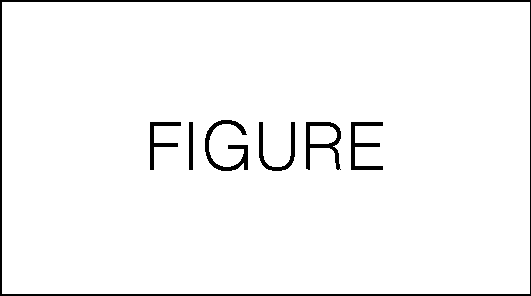
\includegraphics[width=0.7\textwidth]{DRAFT_FigsAndDocs/FIG}
	%%
	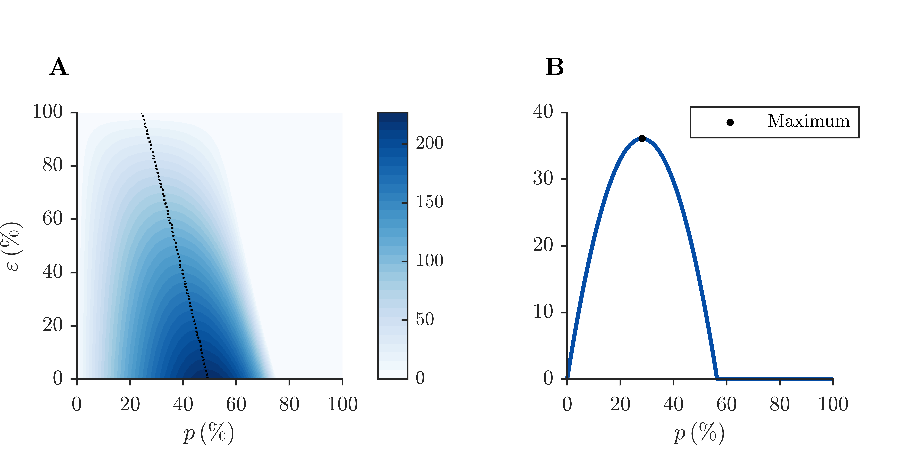
\includegraphics{Figures/PrEP/Results_Baseline/InfectionsOnPrEP}
	\caption[Number of new HIV infections despite PrEP uptake]{%
	{\bf Number of new HIV infections despite PrEP uptake}\\
	The number of new infections among on-PrEP MSM for the baseline scenario, at the endemic state, {\bf (A)} as a function of PrEP coverage ($p$) and PrEP effectiveness ($\varepsilon$), and {\bf (B)} for $\varepsilon=86\%$. For low levels of PrEP coverage, the PrEP-induced risk compensation (i.e., drop on condom use from 30\% to 20\% among PrEP users) outweighs the protection offered by PrEP, and the number of new HIV infections among on-PrEP MSM increases with PrEP coverage. The critical values are depicted by black bullets.}
	\label{fig:InfectionsOnPrEP}
\end{figure}


%%\newpage
%
%\begin{figure}[H]
%	\centering
%	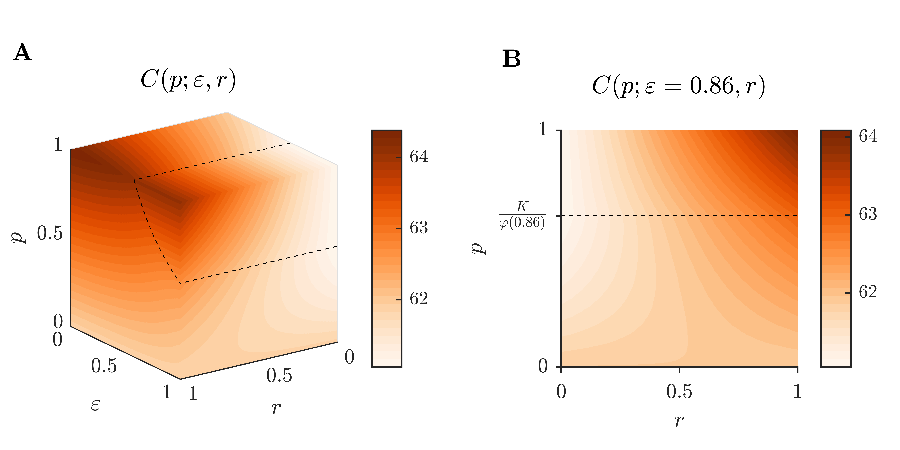
\includegraphics{Figures/PrEP/Cost_4D_cut}
%	\caption[The total expected cost]{%
%	{\bf The total expected cost}\\
%	The total expected cost, $C$, assuming fair risk of HIV infection, for a typical parameter set calibrating our model; see~\hyperlink{Article2SM.8}{eq.~(S25)}. {\bf (A)} $C$ as a function of PrEP coverage ($p$), PrEP effectiveness ($\varepsilon$) and the relative cost of PrEP versus ART ($r$). The total expected cost decreases with increasing PrEP effectiveness $\varepsilon$, and decreasing relative cost $r$. The black dashed line depicts $R(\varepsilon,p)=1$.{\bf (B)} $C$ for a PrEP effectiveness at $\varepsilon = 86\%$. For high relative cost, the total cost $C$ decreases for lower levels of PrEP coverage $p$, while for low relative cost, the total cost $C$ decreases with higher levels of PrEP coverage.
%	}
%	\label{fig:PrEP_C4D}
%\end{figure}


\subsubsection*{The scenario where on-PrEP MSM do not change their HIV testing behavior}
\addcontentsline{toc}{subsubsection}{The scenario where on-PrEP MSM do not change their HIV testing behavior}
\label{sec:FigsSensAnal}

Current guidelines for PrEP prescription require testing for HIV every 3 months~\cite[]{Molina2018}. However, frequent HIV screening may be perceived as a barrier for some individuals~\cite[]{Calabrese2016}. Therefore, frequent HIV testing may not be guaranteed in the long run. We ran our algorithm considering the scenario where MSM do not follow these recommendations, and keep testing for HIV at the same rate than before adopting PrEP (i.e., every $\theta_P=\theta=3.1$ years); cf~\hyperlink{Article2.11}{the sensitivity analyses} of the article and~\hyperlink{Article2.11}{section 3.3.3} of the article's appendix. 

Here, we show the figures analog to those included in the paper and in previous sections, such as the PrEP-induced reduction in HIV incidence (depicted in~\hyperlink{fig:SA_p_hat}{figure \ref*{fig:SA_p_hat}B}), the relative costs thresholds (computed using algorithm~\algoref{algo:rCrE}; see~\figref{fig:SA_r_thresholds}) and the voluntary PrEP coverage resulting from risk misperception (see~\figref{fig:SA_Misperception}), for the scenario where individuals do not change their HIV testing behavior.

We also used $\sim500$ sets of parameters calibrating our model, in order to compute the probability of epidemic elimination (see~\hyperlink{fig:SA_ProbElim}{figure \ref*{fig:SA_ProbElim}A}) and to obtain confidence intervals for the PrEP effectiveness thresholds for epidemic control, $\varepsilon_{\rm C}$, and elimination, $\varepsilon_{\rm E}$ (see~\hyperlink{fig:SA_ProbElim}{figure \ref*{fig:SA_ProbElim}B}). 
%
\hyperlink{fig:SA_ProbElim}{Figure \ref*{fig:SA_ProbElim}C} depicts the relative cost thresholds for epidemic control and elimination, computed numerically for the $\sim500$ parameters sets. Similarly to \secref{sec:Comp_rCrE}, $r_{\rm E}(\varepsilon)$ is the boundary between region II and regions I--IV together. Therefore, for $\varepsilon < \varepsilon_{\rm E}$, we identified $r_{\rm E}(\varepsilon)$ as the highest value of $r$ for which $\hat{p}(\varepsilon,r)=1$; cf. figures~\ref{fig:SA_p_hat} and \hyperlink{fig:SA_ProbElim}{\ref{fig:SA_ProbElim}C}.


%\newpage
\begin{figure}[H]
	\centering
	%% DRAFT
%	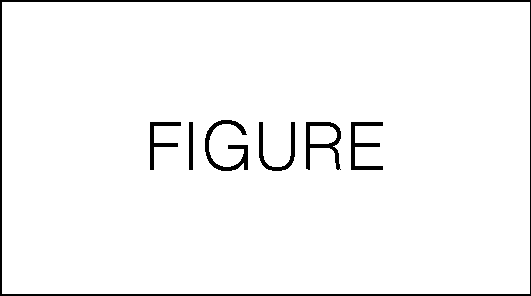
\includegraphics[width=0.7\textwidth]{DRAFT_FigsAndDocs/FIG}
	%%
	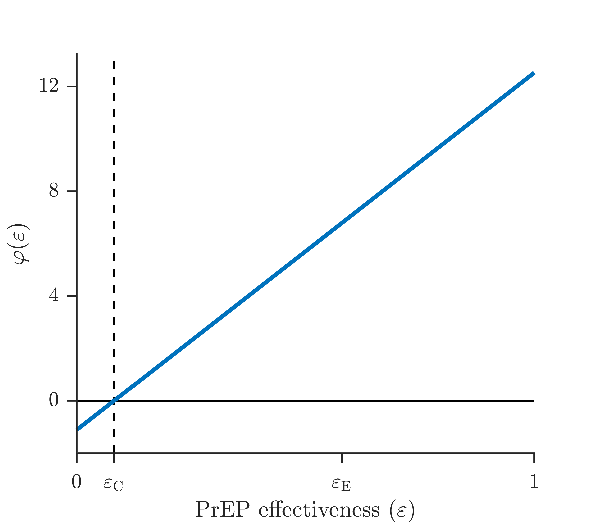
\includegraphics{Figures/PrEP/Results_SensitivityAnalysis/phi}
	\caption[The combined effectiveness of PrEP and condom use, for the scenario where on-PrEP MSM do not change HIV testing behavior]{%
		{\bf The combined effectiveness of PrEP and condom use, for the scenario where on-PrEP MSM do not change HIV testing behavior}\\
	The combined effectiveness of PrEP and condom use among on-PrEP high-risk MSM, relative to the effectiveness of condom use alone among off-PrEP high-risk MSM, $\varphi(\varepsilon)$, when MSM do not change their testing behavior (i.e., $\theta_P=\theta=3.1$ years), for a condom effectiveness of 70\% and a PrEP-induced drop in condom use from 30\% to 20\%; see~\hyperlink{Article2supp.12}{eq.~(S4)} of the article's appendix. As stated in \secref{sec:Comp_EpiElim}, epidemic control induced by PrEP and condom use is possible if and only if $\varphi(\varepsilon) > 0$; that is, if $\varepsilon \geq \varepsilon_{\rm C}$.}
	\label{fig:SA_phi}
\end{figure}


%\newpage
\begin{figure}[H]
	\centering	
	%% DRAFT
%	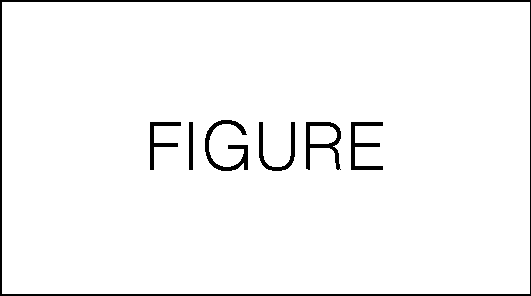
\includegraphics[width=0.9\textwidth]{DRAFT_FigsAndDocs/FIG}
	%%
	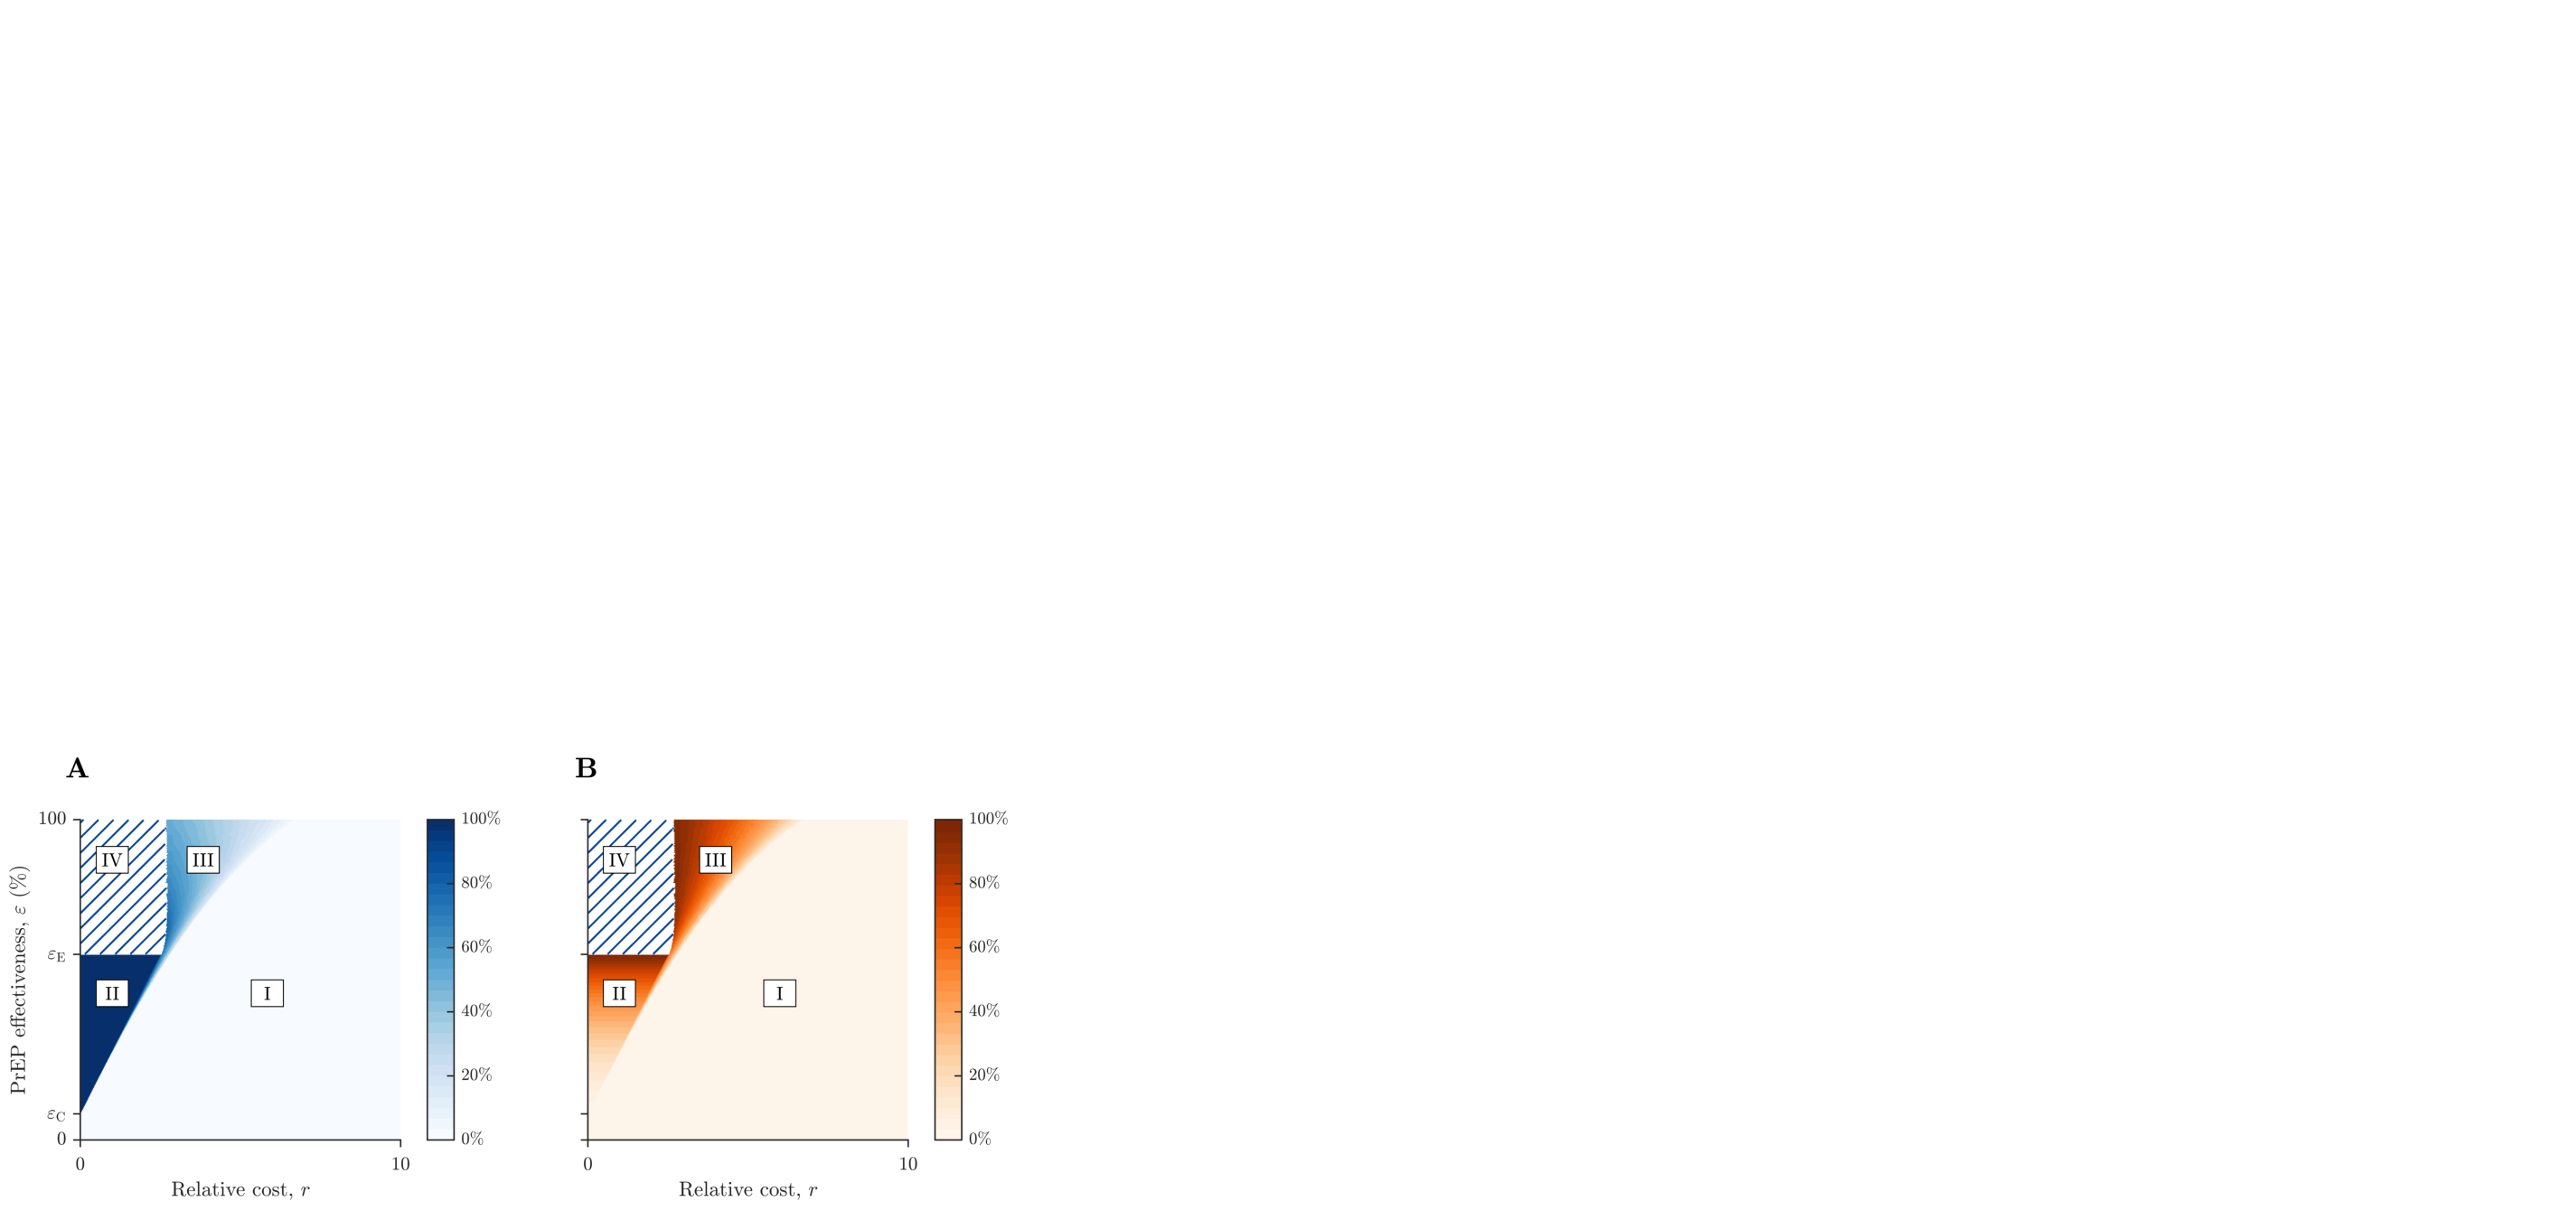
\includegraphics[width=\textwidth]{Figures/PrEP/Results_SensitivityAnalysis/p_hat}
	\caption[The voluntary PrEP coverage and its impact on HIV incidence, for the scenario where on-PrEP MSM do not change HIV testing behavior, assuming fair risk perception]{%
	{\bf The voluntary PrEP coverage and its impact on HIV incidence, for the scenario where on-PrEP MSM do not change HIV testing behavior, assuming fair risk perception} \\
	Color maps of \textbf{(A)} the voluntary PrEP coverage among high-risk MSM ($\hat{p}$) and \textbf{(B)} the corresponding reduction in the overall endemic HIV incidence rate, as functions of $\varepsilon$ and $r$, assuming that individuals have a fair perception of HIV risk and that individuals do not change their testing behaviors once adopting PrEP (i.e., $\theta_P=\theta=3.1$ years). The model outputs were obtained for one typical parameter set calibrating our model. PrEP effectiveness thresholds required to reach epidemic control and epidemic elimination are given by $\varepsilon_{\rm C} = 8\%$ and $\varepsilon_{\rm E} = 58\%$, respectively. Four regions can be identified, depending on the values of $\hat{p}$: region~IV, where all individuals adopt PrEP ($\hat{p}=100\%$) and $\varepsilon_{\rm C} \leq \varepsilon<\varepsilon_{\rm E}$, so the epidemic is controlled; region~III, where no MSM uses PrEP ($\hat{p}=0\%$) and thus, there is no reduction in HIV incidence; region~II, where some, but not enough MSM use PrEP ($0\% < \hat{p} <100\%$) because $r$ remains high and thus the epidemic is controlled; and region~I (marked by blue stripes), where epidemic elimination is possible.}
	\label{fig:SA_p_hat}
\end{figure}


\begin{figure}[H]
	\centering
	%% DRAFT
%	\vspace{1cm}
%	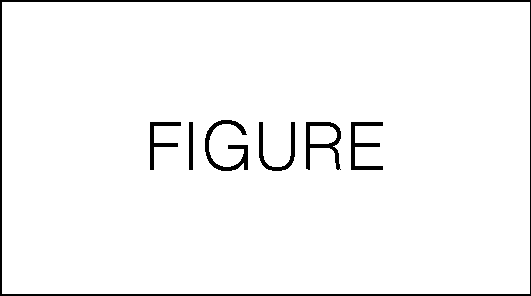
\includegraphics[width=0.7\textwidth]{DRAFT_FigsAndDocs/FIG}
	%%
	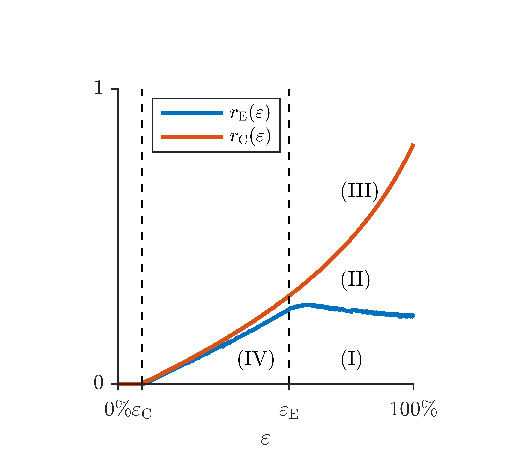
\includegraphics{Figures/PrEP/Results_SensitivityAnalysis/rCrE}
	\caption[The relative cost thresholds for epidemic control and elimination, for the scenario where on-PrEP MSM do not change HIV testing behavior]{%
		{\bf The relative cost thresholds for epidemic control and elimination, for the scenario where on-PrEP MSM do not change HIV testing behavior}\\
	The relative costs thresholds for epidemic control and elimination as functions of PrEP effectiveness (noted $r_{\rm C}(\varepsilon)$ and $r_{\rm E}(\varepsilon)$, respectively), assuming fair perception of the HIV infection risk, for a typical parameter set calibrating our model; see~\hyperlink{Article2supp.12}{table~S4} of the article's appendix. $r_{\rm C}(\varepsilon)$ is the boundary between regions II and region III, while $r_{\rm E}(\varepsilon)$ is the boundary between region II and regions I--VI together. See~\secref{PrEP:Computations} for details on how do we identified these thresholds numerically, from the voluntary PrEP coverage.}
	\label{fig:SA_r_thresholds}
\end{figure}


\begin{figure}[H]
	\centering	
	%% DRAFT
%	\vspace{1cm}
%	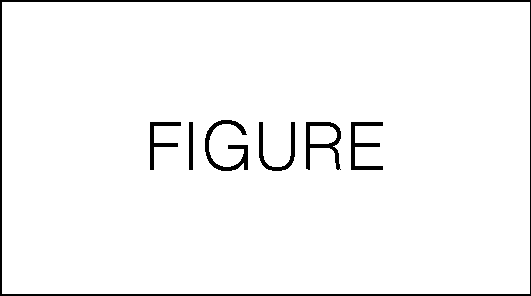
\includegraphics[width=0.7\textwidth]{DRAFT_FigsAndDocs/FIG}
	%%
	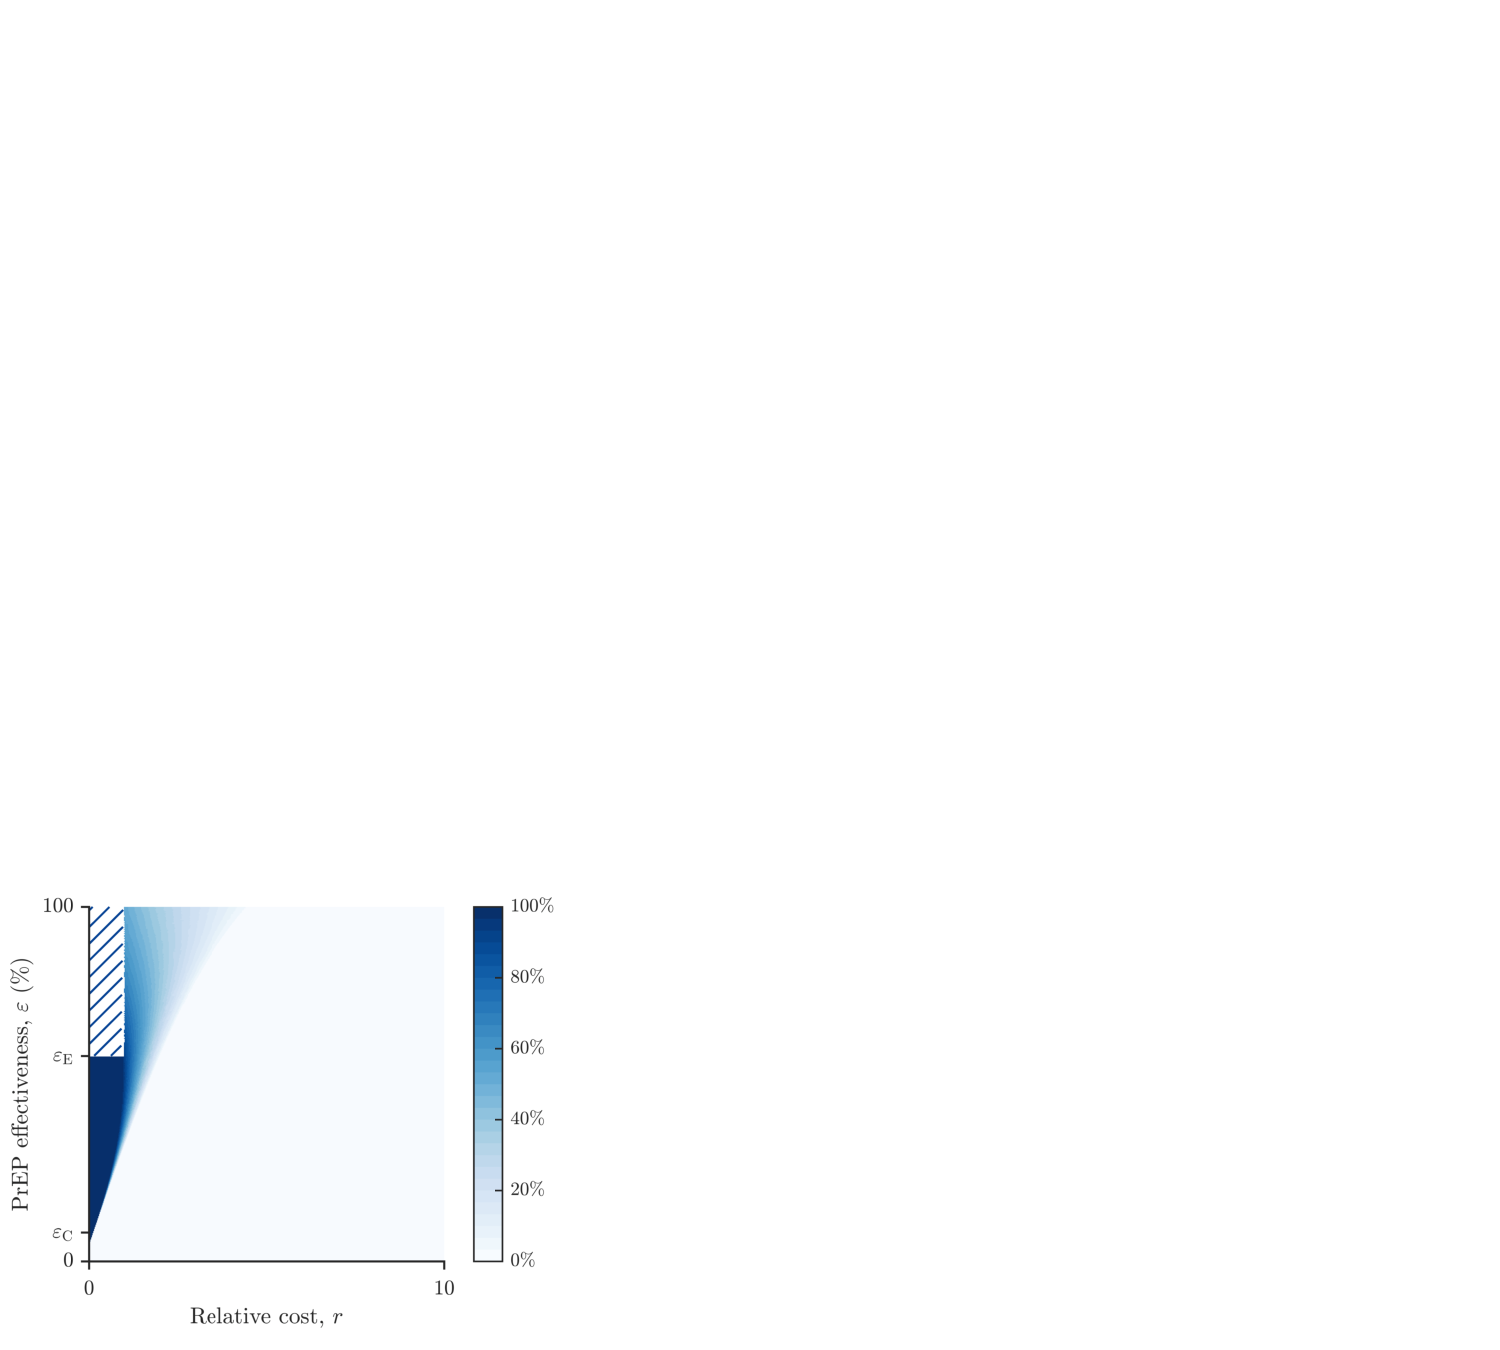
\includegraphics{Figures/PrEP/Results_SensitivityAnalysis/Misperception}
	\caption[The voluntary PrEP coverage, for the scenario where on-PrEP MSM do not change HIV testing behavior, assuming misperception of the HIV infection risk]{%
		{\bf The voluntary PrEP coverage, for the scenario where on-PrEP MSM do not change HIV testing behavior, assuming misperception of the HIV infection risk}\\
	Decision-making based on a misperceived risk of acquiring HIV significantly reduces the size of region~I, where epidemic elimination is possible (blue stripes). The figure was obtained using the same calibrated parameter set as in~\figref{fig:SA_p_hat}. The PrEP effectiveness thresholds for epidemic control and epidemic elimination are, respectively, $\varepsilon_{\rm C} = 8\%$ and $\varepsilon_{\rm E} = 58\%$.}
	\label{fig:SA_Misperception}
\end{figure}


\begin{figure}[H]
	\centering
	%% DRAFT
%	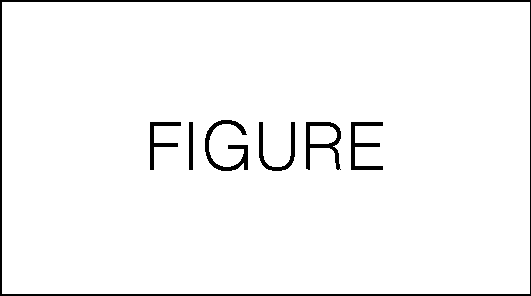
\includegraphics[width=0.6\textwidth]{DRAFT_FigsAndDocs/FIG}
	%%
	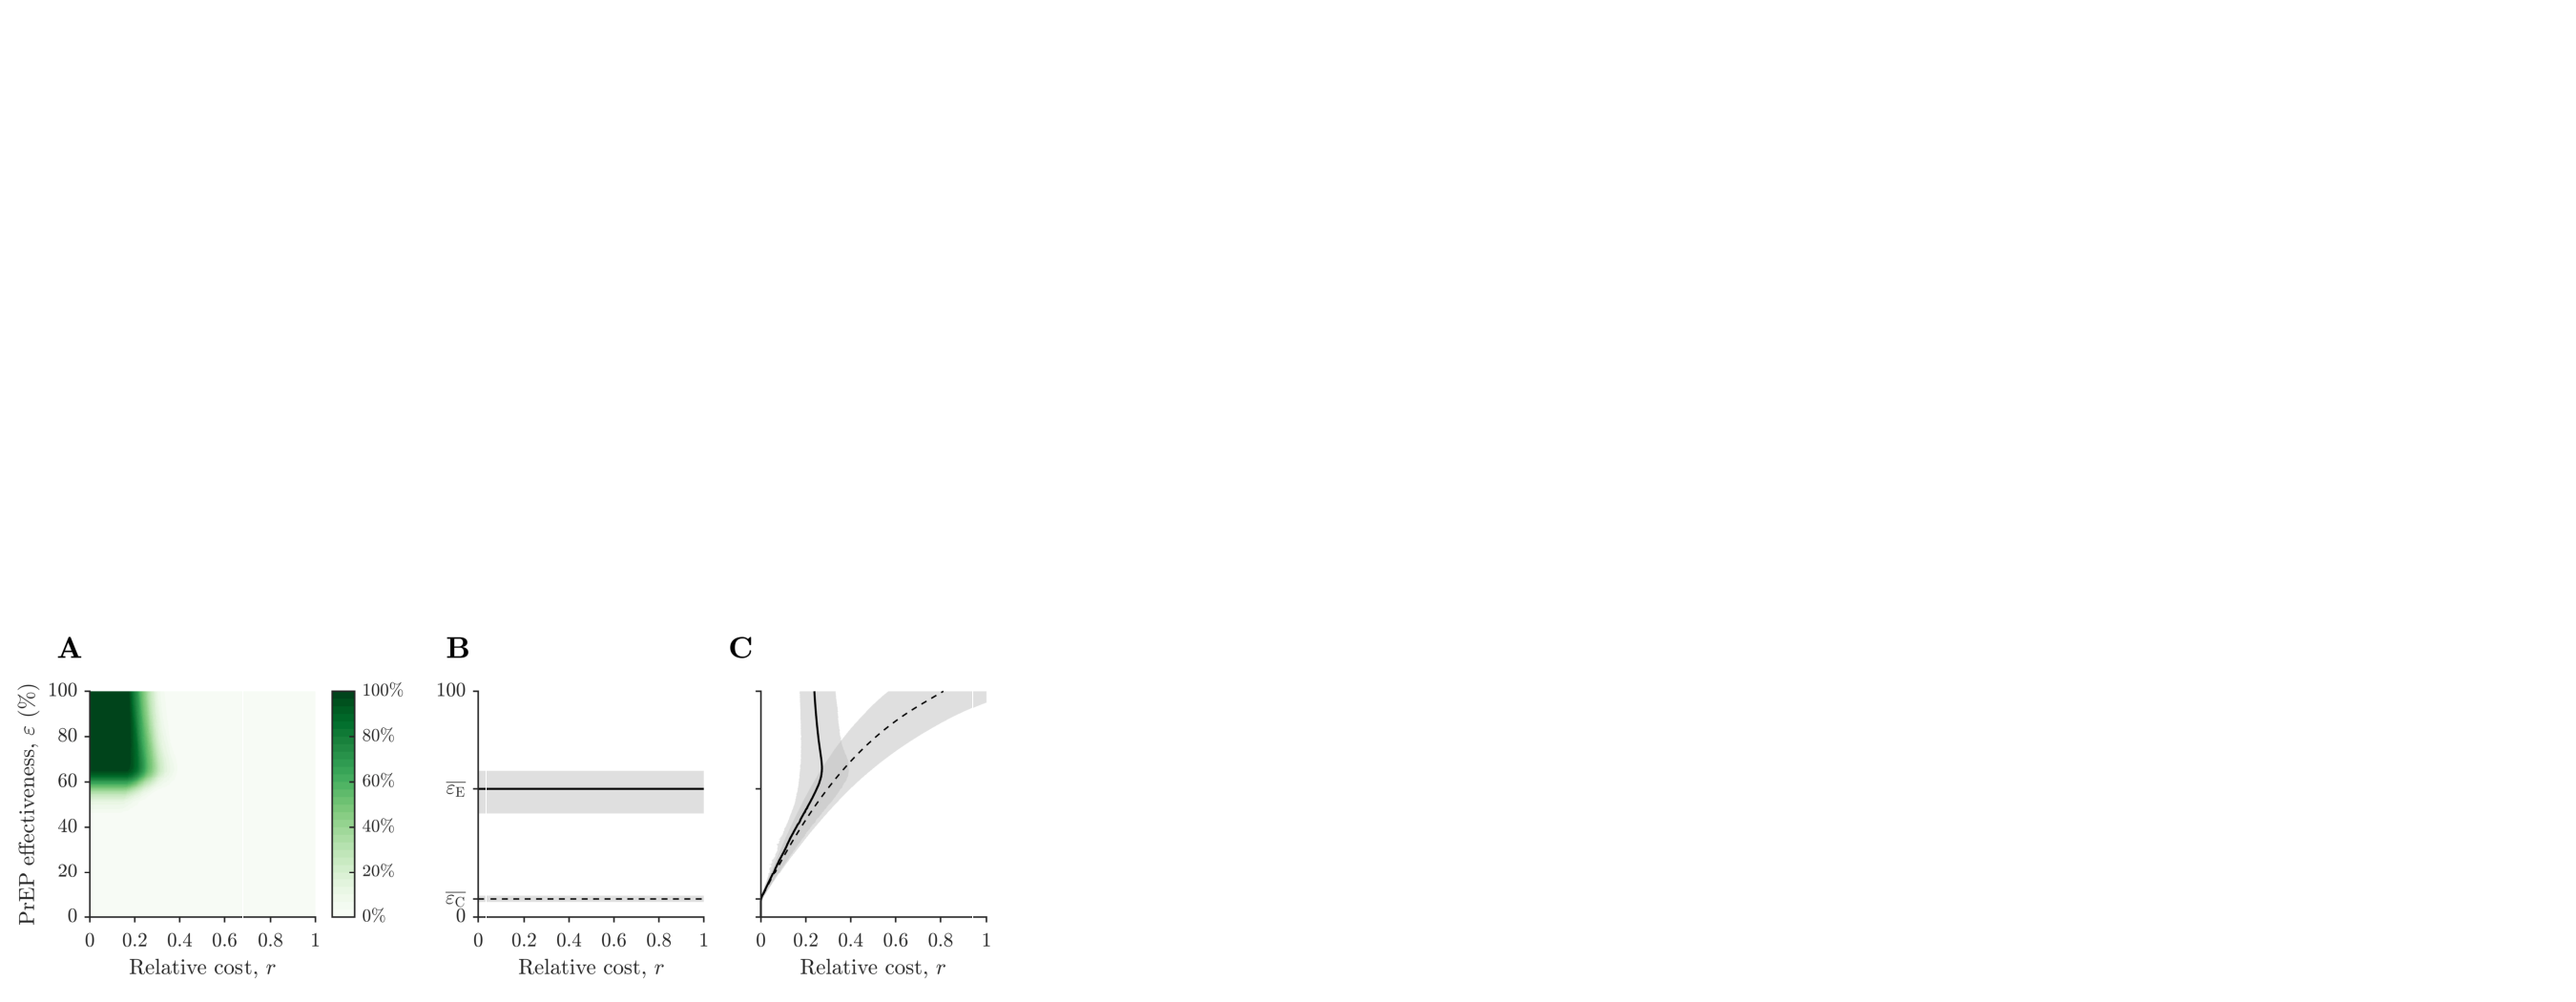
\includegraphics[width=\textwidth]{Figures/PrEP/Results_SensitivityAnalysis/ProbElim}
	\caption[The probability of HIV elimination and boundary uncertainty for the four-regions structure, for the scenario where on-PrEP MSM do not change HIV testing behavior]{%
		{\bf The probability of HIV elimination and boundary uncertainty for the four-regions structure, for the scenario where on-PrEP MSM do not change HIV testing behavior}\\
	\textbf{(A)} The probability of HIV epidemic elimination due to voluntary PrEP coverage, obtained from the $\sim500$ calibrated parameter sets. \textbf{(B)} The mean values for the epidemic control and epidemic elimination thresholds are given by $\varepsilon_{\rm C}=8\%$ (95\%~CI: $7\%$--$9\%$) and $\varepsilon_{\rm E}=57\%$ (95\%~CI: $46\%$--$65\%$), respectively.
	\textbf{(C)} The boundaries (mean and 95\%~CI) between region~II and regions~I and IV (continuous line) and between region~II and region~III (dashed line).}
	\label{fig:SA_ProbElim}
\end{figure}



\section{Further discussion}
\label{PrEP:Discussion}

\subsection{Implementing HIV prevention programs aiming at epidemic elimination}

\subsubsection*{Targeted versus universal PrEP}
\addcontentsline{toc}{subsubsection}{Targeted versus universal PrEP}
Our approach considers the current recommendations, where PrEP is targeted to populations most at risk of HIV infection~\cite[]{WHO_KeyPop2016}. Therefore, in our model, only individuals at high risk of infection may make a decision about PrEP adoption. However, it has been recently discussed to include PrEP into routine prevention healthcare and thus, allowing all sexually active adults to decide whether or not adopt PrEP, in order to improve PrEP adoption by reducing PrEP-related stigma and access inequalities~\cite[]{Calabrese2017}.

%\rev{ET ALORS?}
%Gomez et al. PrEP as a social movement

\subsubsection*{Decreasing the perceived cost of PrEP in the French context}
\addcontentsline{toc}{subsubsection}{Decreasing the perceived cost of PrEP in the French context}
Under our modeling assumptions, high-risk MSM adopting PrEP would be required to maintain high adherence to PrEP for 30 years in average; cf. \hyperlink{Article2SM.16}{Table S2}. According to our results, increasing PrEP coverage among high-risk MSM in France is essential to eliminate HIV transmission among MSM. Even though PrEP is fully reimbursed by the social security system, not enough MSM have adopted PrEP. 

Some difficulties regarding PrEP adoption still need to be addressed. For instance, medical visits are covered only $\sim$70\% by the social security system. In addition, the first PrEP prescription and the yearly renewal must still be done by HIV-specialized doctors working in hospitals or HIV-specialized health centers~\cite[]{HAS_PrEP2019,ANSM_Truvada2020}. This may perpetuate social stigma and discourage some individuals. Training general doctors and allowing them to prescribe PrEP may facilitate and, thus, broaden PrEP access. 

In addition, the healthcare providers' attitudes towards PrEP should be considered. PrEP is currently a medication requiring medical prescription. Hence, an increase in PrEP adoption requires an increase in PrEP prescription. Unfortunately, some healthcare providers may remain reluctant to agree with PrEP use, due to concerns about risk compensation and potential increase in STI transmission~\cite[]{Caumes2018}. As of the end of 2017, STI diagnoses among MSM have significantly increased at the national level~\cite[]{SPF_IST2018}, which could be due to low condom use among the MSM population (and not only among PrEP users). Promoting condom use among MSM may help not only preventing STIs, but also increasing PrEP acceptability. 

%Indeed, an increase in condom use would decrease the risk of infection for on-PrEP MSM, which in turn would decrease the cost associated with the strategy of adopting PrEP to avoid HIV infection (see Eqs.~(\hyperlink{Article2SM.7}{S17}) and~(\hyperlink{Article2SM.7}{S21})).


\subsection{Modeling limitations and perspectives} \label{PrEP:ModelPerspectives}

\subsubsection*{Assuming perfect PrEP adherence}
\addcontentsline{toc}{subsubsection}{Assuming perfect PrEP adherence}
Our model takes into account perfect PrEP adherence. That is, we assume that individuals who adopt PrEP, take PrEP pills correctly, continuously and for life. This assumption may not represent current reality in the Paris region, where only about 85\% of PrEP users got a prescription renewal the following year, since PrEP rollout~\cite[]{ANSM_Truvada2019,ANSM_Truvada2020}. Still, our model may be useful for future presentations of prevention against HIV, such as long-lasting PrEP~\cite[]{} and vaccination~\cite[]{}. Modeling recurrent decision-making~\cite[]{} or the drop of PrEP while being sexually active may be interesting to study.

\subsubsection*{Obtaining data on sexual behavior}
\addcontentsline{toc}{subsubsection}{Obtaining data on sexual behavior}
Including heterogeneity in sexual behavior in modeling studies allows to account for essential behavioral data (for instance, the number of sexual contacts and the proportion of condomless interactions), to which the epidemiology might be very sensitive. However, data on sexual behavior may depend heavily on self-reporting\footnote{It was indeed the case of the data on sexual behavior that we used in our study, collected through the Presse Gays et Lesbiennes survey~\cite[]{Velter2015}}, resulting in high variation of results among some papers~\cite[]{Hess2017}. For instance, there may be some difficulties in obtaining data about the size of the MSM population and the individuals' sexual practices (which gives the population stratification by risk of infection)~\cite[]{Marcus2013b,Baral2018}. Also, data on the number of sexual partners~\cite[]{Hess2017} and most risky contacts might be hard to trace~\cite[]{VanAar2015}. 

Data about stable and occasional relationships~\cite[]{Velter2015} could also be included in the model in order to account for different probabilities of transmission, as well as different probabilities of condom use during the corresponding sexual encounters. This would allow to define the high-risk group not only in terms of the number of sexual contacts but also in terms of the nature of the sexual encounters.

These difficulties point to the importance of better data collection, but also to the importance of fighting stigma around sexual behaviors and preventive methods, so self-declaration becomes more common and reliable. Online tools may help obtaining more and accurate data on sexual behavior~\cite[]{Velter2015,Baral2018}, but population samples may be more biased than those of traditional surveys.

%\subsubsection*{Life expectancy}
%Young, male individuals in high-income settings, who started ART in the period 2008--2013 have an expected age at death of 78~\cite[]{ARTCC2017}.  

\subsubsection*{Targeting other subpopulations}
\addcontentsline{toc}{subsubsection}{Targeting other subpopulations}
Considering risk compensation among non-PrEP users~\cite[]{Phanuphak2018} and explicitly modeling condom use among individuals at low risk of infection might strengthen HIV and other sexually transmitted diseases prevention programs. In addition, considering an age-structured model might help better targeting of high-risk subpopulations, such as young MSM~\cite[]{Siguier2018,WHO_KeyPop2016}. %PrEP among women? (Delabre2021)

\subsubsection*{Considering the heterogeneity in the risk and cost perception}
\addcontentsline{toc}{subsubsection}{Considering the heterogeneity in the risk and cost perception}
In our model, we assumed a homogeneous perception of both the risk of infection and the relative cost of PrEP versus ART, among high-risk MSM. However, in reality, individuals who are eligible to PrEP may perceive their risk of infection and/or the cost of PrEP very differently~\cite[]{Blumenthal2019}. It would be useful to study how the results of our current project change considering heterogeneity in the decision-making and the implications for PrEP rollouts. %This is the objective of a follow-up paper we intend to work on, next.

%\subsubsection*{Using multi-players games}
%Multi-players games can be used to model individuals' strategies about prevention adoption depending on the decision made by the current partner, regarding PrEP and condom use negotiation.

